\documentclass{l4proj}
\usepackage{pdfpages} 
\usepackage{tikz}
\usepackage{float}
\usepackage{enumitem}

\lstdefinelanguage{TML}{ 
    keywords={changeto, move, goto, if, switch, while, module, accept, reject, alphabet},
    ndkeywords={left, right, tapehead, blank},
    sensitive=true,
    comment=[l]{//},
    morecomment=[s]{/*}{*/},
    morestring=[b]',
    morestring=[b]"
}

\newtheorem{theorem}{Theorem}

\begin{document}

\title{Turing Machine Language} 
\author{Pete Gautam}

\maketitle

\begin{abstract}
    % Every abstract follows a similar pattern. Motivate; set aims; describe work; explain results.
    % \vskip 0.5em
    % ``XYZ is bad. This project investigated ABC to determine if it was better. 
    % ABC used XXX and YYY to implement ZZZ. This is particularly interesting as XXX and YYY have
    % never been used together. It was found that  
    % ABC was 20\% better than XYZ, though it caused rabies in half of subjects.''
\end{abstract}

\chapter*{Acknowledgements}
% Enter any acknowledgements here. This is optional; you may leave this blank if you wish,
% or remove the entire chapter
%
% We give thanks to the Gods of LaTeX, who in their eternal graciousness, 
% have granted that this document may compile without errors or overfull hboxes.
%

%==============================================================================

\def\consentname {Pete Gautam} 
\def\consentdate {27 September 2022} 
\educationalconsent

\tableofcontents

\chapter{Introduction}

% reset page numbering. Don't remove this!
\pagenumbering{arabic} 

\section{Motivation}
Turing Machines are a model of computation that is typically taught to computing students after some years of coding experience. They are normally taught the concept using finite state machines. This is quite different to how they have been taught programming previously, and they might find it easier to learn the concept in a way that resembles coding closely. This project presents a language to represent TMs.

\section{Objectives}
There are 3 parts to the project:
\begin{enumerate}
    \item defining the language, 
    \item creating the parser for the language and 
    \item creating a website that allows a user to make use of the parser.
\end{enumerate}

The first aim is to define a programming language to represent Turing machines, called the Turing Machine Language. A Turing machine can be executed on a tape, and this is what the language will simulate. 

Next, a parser will be created for the language. This parser should be able to take in a string representation of a program, and then parse it into a program context. Then, a program context can be:
\begin{itemize}
    \item validated to ensure it has no errors;
    \item converted into a Turing machine; and
    \item executed on a tape.
\end{itemize}

Finally, a website will be created to allow the user to access the parser. It should feature an editor to allow users to type a program. The user would then be able to convert it into a Turing machine, or execute it on a valid tape.

\section{Summary}
TODO

% \todo{Remove the guidance notes from your dissertation before submitting!}

% Why should the reader care about what are you doing and what are you actually doing?
% \section{Guidance}

% \textbf{Motivate} first, then state the general problem clearly. 

% \section{Writing guidance}
% \subsection{Who is the reader?}

% This is the key question for any writing. Your reader:

% \begin{itemize}
%     \item
%     is a trained computer scientist: \emph{don't explain basics}.
%     \item
%     has limited time: \emph{keep on topic}.
%     \item
%     has no idea why anyone would want to do this: \emph{motivate clearly}
%     \item
%     might not know \emph{anything} about your project in particular:
%     \emph{explain your project}.
%     \item
%     but might know precise details and check them: \emph{be precise and
%     strive for accuracy.}
%     \item
%     doesn't know or care about you: \emph{personal discussions are
%     irrelevant}.
% \end{itemize}

% Remember, you will be marked by your supervisor and one or more members
% of staff. You might also have your project read by a prize-awarding
% committee or possibly a future employer. Bear that in mind.

% \subsection{References and style guides}
% There are many style guides on good English writing. You don't need to
% read these, but they will improve how you write.

% \begin{itemize}
%     \item
%     \emph{How to write a great research paper} \cite{Pey17} (\textbf{recommended}, even though you aren't writing a research paper)
%     \item
%     \emph{How to Write with Style} \cite{Von80}. Short and easy to read. Available online.
%     \item
%     \emph{Style: The Basics of Clarity and Grace} \cite{Wil09} A very popular modern English style guide.
%     \item
%     \emph{Politics and the English Language} \cite{Orw68}  A famous essay on effective, clear writing in English.
%     \item
%     \emph{The Elements of Style} \cite{StrWhi07} Outdated, and American, but a classic.
%     \item
%     \emph{The Sense of Style} \cite{Pin15} Excellent, though quite in-depth.
% \end{itemize}

% \subsubsection{Citation styles}

% \begin{itemize}
% \item If you are referring to a reference as a noun, then cite it as: ``\citet{Orw68} discusses the role of language in political thought.''
% \item If you are referring implicitly to references, use: ``There are many good books on writing \citep{Orw68, Wil09, Pin15}.''
% \end{itemize}

% There is a complete guide on good citation practice by Peter Coxhead available here: \url{http://www.cs.bham.ac.uk/~pxc/refs/index.html}. 
% If you are unsure about how to cite online sources, please see \citet{UNSWWebsite}. 
% \footnote{Specifying an online resource like \url{https://developer.android.com/studio}
% in a footnote sometimes makes more sense than including it as a formal reference.}

% \subsection{Plagiarism warning}

% \begin{highlight_title}{WARNING}
    
%     If you include material from other sources without full and correct attribution, you are commiting plagiarism. The penalties for plagiarism are severe.
%     Quote any included text and cite it correctly. Cite all images, figures, etc. clearly in the caption of the figure.
% \end{highlight_title}

% \subsection{Quoting text}

% If you are quoting a long passage, use a \texttt{quote} environment:

% \begin{quote}
%      If you scribble your thoughts any which way, your readers will surely feel that you care nothing about them. They will mark you down as an egomaniac or a chowderhead -or, worse, they will stop reading you. The most damning revelation you can make about yourself is that you do not know what is interesting and what is not.
% \end{quote} \citep{Von80}

% If you are quoting inline, like Simon Peyton-Jones' following remark, use quotation marks ``Conveying the intuition is primary, not
% secondary'' \citep{Pey17}.


\chapter{Background}
\section{Turing Machine}
\subsection{Introduction to Turing Machines}
A \emph{Turing Machine} (TM) is a collection $(Q, \Sigma, \delta, q_0)$, where:
\begin{itemize}
    \item $Q$ is a set of \emph{states}, including the \emph{accept state} $A$ and \emph{reject state} $R$;
    \item $\Sigma$ is the set of \emph{letters}, which does not include the \texttt{blank} symbol;
    \item $\delta \colon Q \setminus \{A, R\} \times \Sigma^+ \to Q \times \Sigma^+ \times \{\texttt{left}, \texttt{right}\}$, where $\Sigma^+ = \Sigma \cup \{\texttt{blank}\}$, is the \emph{transition function}; and
    \item $q_0 \in Q$ is the \emph{starting state}.
\end{itemize}
Although based on Turing's work on \cite{turing1936computable}, this definition, along with others in this section, have been adapted from \cite{hopcroft2001automata}.

\begin{figure}[htb]
    \centering
    \begin{subfigure}{0.45\textwidth}
        \centering
        \begin{tikzpicture}
            \node[state, accepting] (q0) at (0, 0) {$q_0$};
            \node[state] (q1) at (2.5, 0) {$q_1$};
            \node[state, fill=green, opacity=0.6] (A) at (5, -1) {$A$};
            \node[state, fill=red, opacity=0.6] (R) at (5, 1) {$R$};
    
            \draw[->] (q0) edge[loop above] node[text width=1.5cm, align=center] {$0 \to 0, R$ $1 \to 1, R$} (q0);
            \draw[->] (q0) -- node[above] {$\# \to \#, L$} (q1);
            \draw[->] (q1) -- node[below, rotate=-20] {$0 \to \#, L$} (A);
            \draw[->] (q1) -- node[above, rotate=20, text width=1.5cm, align=center] {$1 \to 1, L$ $\# \to \#, L$} (R);
        \end{tikzpicture}
        \caption{Full notation}
    \end{subfigure}
    \hfill
    \begin{subfigure}{0.45\textwidth}
        \centering
        \begin{tikzpicture}
            \node[state, accepting] (q0) at (0, 0) {$q_0$};
            \node[state] (q1) at (2.5, 0) {$q_1$};
            \node[state, fill=green, opacity=0.6] (A) at (5, -1) {$A$};
            \node[state, fill=red, opacity=0.6] (R) at (5, 1) {$R$};
    
            \draw[->] (q0) edge[loop above] node {$0|1, R$} (q0);
            \draw[->] (q0) -- node[above] {$\#, L$} (q1);
            \draw[->] (q1) -- node[below, rotate=-20] {$0 \to \#, L$} (A);
            \draw[->] (q1) -- node[above, rotate=20] {$1|\#, L$} (R);
        \end{tikzpicture}
        \caption{Shorthand notation}
    \end{subfigure}
    \caption{A FSM representation of a TM that accepts binary numbers divisible by 2.}
    \label{fig:tm_isDiv2}
\end{figure}

We can represent a TM as a finite state machine (FSM). This is a directed graph, with vertices as states and edges as transitions. An example is given in Figure \ref{fig:tm_isDiv2}. In this case, the alphabet $\Sigma = \{0, 1\}$. The blank symbol is denoted by $\#$. The initial state is denoted by $q_0$; the accept state $A$ and the reject state $R$. Every edge corresponds to an evaluation of the transition function $\delta$, e.g. $\delta(q_1, 0) = (A, \texttt{blank}, \texttt{left})$. 

The figure presents two ways of representing a FSM- subfigure (a) shows all the transitions, while subfigure (b) only shows the transitions where the tapehead value is getting changed. It also combines certain letters if they are not being changed. We will make use of the shorthand FSM representation from now.

\subsection{Executing a TM on a tape}
Let $\Sigma$ be an alphabet. A \emph{tape} $T$ on $\Sigma$ is a function $T\colon \mathbb{Z} \to \Sigma^+$. In particular, the tape has infinite entries in both directions. 

\begin{figure}[htb]
    \centering
    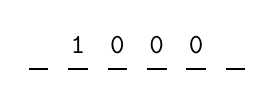
\begin{tikzpicture}
        \foreach \x[count=\i] in {, 1, 0, 0, 0, } {
            \draw[thick] (\i*0.5-0.25, 0) -- (\i*0.5, 0);
            \node at (\i*0.5-0.125, 0.3) {\texttt{\x}};
        }
    \end{tikzpicture}
    \caption{A TM tape on $\{0, 1\}$.}
    \label{fig:tape_example}
\end{figure}
We can represent a tape using a figure. For instance, let $\Sigma = \{0, 1\}$, and let $T$ be the tape on $\Sigma$ given below:
\[T(x) = \begin{cases}
    0 & x \in \{0, 2, 3\} \\
    1 & x \in \{1\} \\
    \texttt{blank} & \text{otherwise}.
\end{cases}\]
Then, Figure \ref{fig:tape_example} represents the tape $T$. We will assume that the first non-blank value is at index 0.

We can execute a TM on a tape. Let $M$ be a TM with alphabet $\Sigma$, and let $T$ be a tape on $\Sigma$. We execute $M$ on $T$ inductively, as follows:
\begin{itemize}
    \item At any point during execution, we maintain 3 objects:
    \begin{enumerate}
        \item a tape on $\Sigma$, 
        \item a (current) state in $M$ and 
        \item an index in the tape (called the \emph{tapehead index}). 
    \end{enumerate}
    
    \item At the start,
    \begin{enumerate}
        \item the tape is $T$; 
        \item the tapehead index is $0$; and
        \item the current state is the initial state $q_0$. 
    \end{enumerate}
    
    \item At some point during the execution, assume that we have the tape $S$, tapehead index $j$, with \emph{tapehead value} $T(j) = t$, and a non-terminating state $q$ (i.e. not $A$ or $R$). Denote $\delta(q, t) = (q', t', \texttt{dir})$. Then, 
    \begin{enumerate}
        \item the next state is $q'$;
        \item the next tape is $S'$, where
        \[S'(x) = \begin{cases}
            t' & x = i \\
            S(x) & \text{otherwise};
        \end{cases}\]
        and
        \item the next tapehead index is $j'$, where
        \[j' = \begin{cases}
            j+1 & \texttt{dir} = \texttt{right} \\
            j-1 & \texttt{dir} = \texttt{left}.
        \end{cases}\]
    \end{enumerate}
    If the state $q'$ is not a terminating state, then the execution continues with these 3 objects. Otherwise, execution is terminated with terminating state $q'$.
\end{itemize}

We illustrate this process with the TM in Figure \ref{fig:tm_isDiv2} with the tape in Figure \ref{fig:tape_example}:
\begin{itemize}
    \item Initially, 
    \begin{enumerate}
        \item the tape is the given tape;
        \item $q_0$ is the current state; and 
        \item the tapehead index is $0$, with value $1$.
    \end{enumerate}
    \item According to the FSM, we have $\delta(q_0, 1) = (q_0, 1, R)$. Hence,
    \begin{enumerate}
        \item the tape remains unchanged;
        \item $q_0$ is still the current state; and
        \item and the tapehead index becomes $1$, with value is \texttt{0}.
    \end{enumerate}
    \item The transition for \texttt{0} and \texttt{1} are the same with respect to $q_0$. This means that we keep moving to the right until we end up at a blank symbol. At that point, the following is the state of the tape:
    \begin{figure}[H]
        \centering
        \begin{tikzpicture}
            \foreach \x[count=\i] in {, 1, 0, 0, 0, } {
                \draw[thick] (\i*0.5-0.25, 0) -- (\i*0.5, 0);
                \node at (\i*0.5-0.125, 0.3) {\texttt{\x}};
            }
            \draw[->] (2.875, -0.5) -- (2.875, -0.1);
        \end{tikzpicture}
    \end{figure}
    The arrow points at the tapehead value. We are still at the state $q_0$, and the tape has not been altered.
    
    \item Now, since the tapehead value is \texttt{blank}, we move to the left and the current state becomes $q_1$. The tape has still not been changed. The current value is now $0$.
    
    \item We have $\delta(q_1, 0) = (A, \texttt{blank}, L)$. So, 
    \begin{enumerate}
        \item the tapehead value changes to from $0$ to blank;
        \item the current state becomes $A$; and
        \item the tapehead pointer move to the left, at index $2$.
    \end{enumerate}
    Since $A$ is a terminating state, execution terminates, with result accept. The final tape state is the following:
    \begin{figure}[H]
        \centering
        \begin{tikzpicture}
            \foreach \x[count=\i] in {, 1, 0, 0, , } {
                \draw[thick] (\i*0.5-0.25, 0) -- (\i*0.5, 0);
                \node at (\i*0.5-0.125, 0.3) {\texttt{\x}};
            }
            \draw[->] (1.875, -0.5) -- (1.875, -0.1);
        \end{tikzpicture}
    \end{figure}
\end{itemize}
So, the TM works as follows:
\begin{itemize}
    \item we use the state $q_0$ to traverse to the first blank symbol (i.e. the end of the string), and then move to the state $q_1$;
    \item at state $q_1$, we accept the string if and only if the current tapehead value is \texttt{0}
\end{itemize}
Hence, this TM accepts binary numbers if and only if they are divisible by 2.

\subsection{TM as a model of computation}
Turing initially proposed TMs as the `correct' model of computation in \cite{turing1936computable}. This result is referred to as the \emph{Church-Turing Thesis}. It is a thesis since it is informal in nature; it is just a \textit{belief} that the correct model of computation is the model generated by TMs. 

In this paper, he also showed that TMs and $\lambda$-calculus are equivalent to TMs. Hence, he showed that $\lambda$-calculus is also the correct model of computation. There have been many other models of computations proposed, such as general recursive functions. It is widely regarded that TMs (and all the equivalent models) represent the correct model of computation. This is because many of the originally proposed models of computation turned out to be equivalent (\cite{copeland2004essential}).

\section{Parser}
A \emph{compiler} is a program that takes source code in a programming language (PL) and translates it into a program in another, target, PL. During the process, the compiler also detects any errors, such as syntax and type errors. 

\begin{figure}[htb]
    \centering
    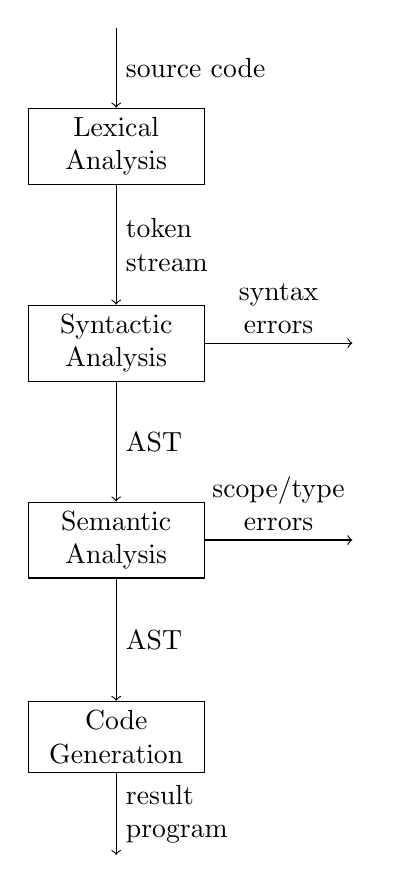
\begin{tikzpicture}
        \node[draw, text width=2cm, align=center] (LA) at (0, 0) {Lexical Analysis};
        \node[draw, text width=2cm, align=center] (SA) at (0, -2.5) {Syntactic Analysis};
        \node[draw, text width=2cm, align=center] (CA) at (0, -5) {Semantic Analysis};
        \node[draw, text width=2cm, align=center] (CG) at (0, -7.5) {Code \\ Generation};
        
        \draw[->] (0, 1.5) -- node[right] {source code} (LA);
        \draw[->] (LA) -- node[right, text width=2cm, align=left] {token \\ stream} (SA);
        
        \draw[->] (SA) -- node[above, text width=2cm, align=center] {syntax \\ errors} (3, -2.5);
        \draw[->] (SA) -- node[right] {AST} (CA);
        \draw[->] (CA) -- node[above, text width=2cm, align=center] {scope/type \\ errors} (3, -5);
        
        \draw[->] (CA) -- node[right] {AST} (CG);
        \draw[->] (CG) -- node[text width=2cm, align=left, right] {result \\ program} (0, -9);
    \end{tikzpicture}
    \caption{The data flow between the compilation phases.}
    \label{fig:compilation_process}
\end{figure}

We will now consider the different phases of the compilation process. This is summarised in Figure \ref{fig:compilation_process}. This figure, along with most of the content in this section, has been adapted from \cite{aho2007compilers}.

\subsection{Lexical Analysis}    
First, we perform \emph{lexical analysis}. In this stage, the source code is enriched to make it ready for parsing. In particular, we generate a stream of source code, which reads the program word by word. Then, it produces a stream of \emph{tokens}. A token is a word in source code along with a label. For instance, consider the mathematical expression \texttt{1 + 2}. We can convert this expression into 3 tokens: \texttt{(1, NUM)}, \texttt{(+, PLUS)} and \texttt{(2, NUM)}. 

\subsection{Syntactic Analysis}
Next, we try to parse the token stream into an (abstract) syntax tree (AST). If there are syntax errors present in the program, then it is not possible to construct a syntax tree. This will be detected during this phase, at which point we can throw a syntax error.

A syntax tree represents the program as a tree of nodes. Typically, the internal nodes represent operations and the leaves represent their arguments. An AST is a compact representation of a syntax tree that does not feature all the nodes. The abstract syntax tree for the expression \texttt{(1 + 2) * (3 + 4)} is given in Figure \ref{fig:AST_example}.

\begin{figure}[htb]
    \centering
    \begin{tikzpicture}[
        level 1/.style={sibling distance=4cm},
        level 2/.style={sibling distance=2cm},
    ]
        \node[ellipse, draw] {TIMES}
        child {
            node[ellipse, draw] {PLUS}
            child {
                node[draw] {\texttt{1}}
            }
            child {
                node[draw] {\texttt{2}}
            }
        }
        child {
            node[ellipse, draw] {PLUS}
            child {
                node[draw] {\texttt{3}}
            }
            child {
                node[draw] {\texttt{4}}
            }
        };
    \end{tikzpicture}
    \caption{The AST for the expression \texttt{(1 + 2) * (3 + 4)}}
    \label{fig:AST_example}
\end{figure}

There are many ways to parse the stream of tokens. A common method is \emph{recursive-descent} parsing. Here, we recursively parse the source code and generate nodes within the AST. For instance, we initially start by parsing a program. If we then encounter an expression, and this is allowed in the grammar of the language, we parse an expression. 

One way of recursive-descent parsing is by \emph{top-down} parsing. In this case, we produce the parent node of the AST and then generate its children. 

The simplest form of recursive-descent parsing is called \emph{predictive parsing}. This applies when the next token determines what structure it is to be parsed. For instance, if we see the token \texttt{if}, then we know we are parsing an \textit{if} command. Such a parser makes use of the \texttt{match} method- this is used to match the next token value.

% A snippet of a recursive-descent class \texttt{CodeParser} is given below, which illustrates how an if statement might be parsed.
% \begin{lstlisting}[language=TypeScript]
% class CodeParser {
%     parseIf():IfContext {
%         match("if");
%         var condition = parseExpr();
        
%         match("then");
%         var expr1 = parseExpr();
        
%         match("else");
%         var expr2 = parseExpr();

%         return new IfContext(condition, expr1, expr2);
%     }

%     // ... other parsing methods
% }
% \end{lstlisting}

\subsection{Semantic Analysis}
Now, we traverse the AST and check that there were no errors in the source code. Typically, there are 2 types of things to check in this stage- type and scope errors. 

In type errors, we check whether the AST has some type mismatch, e.g. \texttt{1 + true}. If there are no errors, then we will have assigned types to each variable. This information will likely be used during code generation.

In scope errors, we check whether some identifier present in code is undefined. To do so, we need to keep track of all the variables that are in scope at this point. In terms of functions, there is a design choice here- we can have all functions in scope from the start, or add them to scope as they are encountered. 

\subsection{Code Generation}
Finally, we convert the AST into code in the target language. In particular, we traverse the tree left-to-right and convert each phrase from the source language to the target. This can also be done using the visitor design pattern. Here, the return type is expected to be a representation of the target language.

\chapter{Requirements}

MoScoWs were used to specify the requirements for the project. In particular, the requirements were partitioned into one of the 4 levels of priority:
\begin{itemize}
    \item \emph{must have} this feature is required to construct the minimum viable product; 
    \item \emph{should have} this feature is required for the product to be practically useful;
    \item \emph{could have} this feature is a stretch goal but is plausible; and
    \item \emph{will not have} this feature is not something that can be implemented in the given time (or conflicts with another feature).
\end{itemize} 
Since the project has 3 distinct aspects, each part had its own MoScoW section. Both functional and non-functional requirements are given together.

\section{Turing Machine Language}
\begin{itemize}
    \item A specification document for the Turing Machine Language (TML) \emph{must} be created.
    \item A proof of equivalence between TMs and TML programs \emph{must} be provided. 
    \item The language \emph{must} abstract details of TM, such as states and transitions.
    \item The language \emph{must not} abstracting execution on tape, e.g. we can only move one step to the left or right during execution.
    \item The language \emph{should} resemble a traditional programming language.
    \item The specification \emph{should} include a formal and an informal definition for the language.
    \item The specification \emph{should} include how to execute a program on a valid tape.
    \item The specification \emph{should} include examples of programs \textit{before} definitions and proofs. \textit{This is so that the document is easier to follow}.
    \item The specification and proof \emph{could} connect TML program with the Church-Turing Thesis. 
\end{itemize}

\section{Developing the parser for TML}
\begin{itemize}
    \item The parser \emph{must} be correct.
    \item The parser \emph{must} support web deployment. 
    \item The parser \emph{must} be able to parse a string representation of a TM program to a program context.
    \item The parser \emph{must} be able to validate a program context.
    \item The parser \emph{must} be able to execute a program context on a valid tape.
    \item The parser \emph{should} be able to convert a program context to a TM. \textit{Compared to the 3 must-have requirements, this requirement was considered to be of the lowest priority, and so was considered a should-have.}
    \item The parser \emph{could} be able to execute a TM on a tape. \textit{This might help in the website to illustrate execution on the converted TM.}
    \item The parser \emph{will not} be able to convert a TM into a TML program.
\end{itemize}

\section{The Product}

\begin{figure}[htb]
    \centering
    \begin{tikzpicture}
        \node[state, accepting] (q0) at (0, 0) {$q_0$};
        \node[state] (q1) at (2.5, 0) {$q_1$};
        \node[state, fill=green, opacity=0.6] (A) at (5, 0) {$A$};
        \node[state, fill=red, opacity=0.6] (R) at (7.5, 0) {$R$};

        \draw[->] (q0) edge[loop above] node {$0|1, R$} (q0);
        \draw[->] (q0) -- node[above] {$\#, L$} (q1);
        \draw[->] (q1) -- node[above] {$0, L$} (A);
        \draw[->] (q1) -- node[above, pos=0.75] {$1|\#, L$} (R);
    \end{tikzpicture}
    \caption{A possible initial rendering of a FSM}
    \label{fig:bad_FSM}
\end{figure}

\begin{itemize}
    \item The website \emph{must} have a code editor for TML.
    \item The website \emph{must} be able to convert a valid program to a TM and present it as a FSM.
    \item The website \emph{must} be able to execute a program on a valid tape, one step at a time.
    \item The code editor \emph{should} support syntax highlighting.
    \item The user should be able to drag states within the FSM. \textit{This is under the assumption that the website does not make use of any fancy FSM assignment algorithm, i.e. it would produce an initial rendering of FSM such as the one in Figure \ref{fig:bad_FSM}.}
    \item The website \emph{should} be fast, easy to use, responsive and well-designed.
    \item The website \emph{should} be accessible by both laptops and tablets.
    \item The website \emph{should} include documentation. \textit{This is to allow people with little or no knowledge of TMs to use the site. Also, the TML is a new concept, so people using the site are not necessarily going to be familiar with it!}
    \item The editor \emph{could} support error detection.
    \item The user \emph{could} be able to configure the website, e.g. change the editor theme, the editor font size and the speed of tape execution. 
    \item The website \emph{could} convert a program to its definition as a TM. 
    \item The website \emph{could} support automatic placement of states within the FSM in an aesthetic manner.
    \item The editor \emph{will not} be able to automatically fix errors.
    \item The website \emph{will not} be able to directly execute a TM on a tape. 
    \item The website \emph{will not} able to convert a TM into a TML program.
    \item The website \emph{will not} be accessible on phones.
\end{itemize}


\chapter{Design}
\section{Language}

The TML provides commands to specify tape operations. In particular, 
\begin{itemize}
    \item we make use of \texttt{move} commands to move the tapehead pointer in some direction; and
    \item we make use of \texttt{changeto} commands to change the tapehead value to some letter in the alphabet.
\end{itemize}
To abstract states in a TM, the TML provides a PL-like alternative, called \emph{modules}. A module simulates a state in TMs. To allow for flow of code to go from one module to another, we make use of \texttt{goto} commands. We can go to the \textit{accept} and \textit{reject} states using the keywords \texttt{accept} and \texttt{reject} respectively.

The following illustrates a simple program in TML with all the basic operations.
\lstinputlisting[language=TML]{code/simple_program.txt}
The execution of a program starts at the first module, i.e. the module \texttt{first}. We remove the first tape value and move the tape pointer to the right. We then go to module \texttt{second} and continue execution. Note that we allow recursion- line 5 can be replaced with \texttt{goto first}.

To abstract the transition function, the language makes use of \emph{pattern-matching}. To resemble a traditional PL, we make use of \texttt{if} commands. This is shown in the example below.
\lstinputlisting[language=TML]{code/pattern_matching.txt}

Although the language is already equivalent to TMs, TML programs do not abstract TMs enough. In particular, modules are equivalent to TM states at this point. To mitigate this, we add nesting within \texttt{if} statements. That way, modules are more expressible than states. It also allows us to write programs that are more comparable to programs written in other languages. An example of a nested TML program is given below.
\lstinputlisting[language=TML]{code/isDiv2Rec.txt}
In this program, we have nested an \texttt{if} block within an \texttt{if} block in lines 12-16.

\begin{figure}[htb]
    \centering
    \begin{tikzpicture}
        \node[state, accepting] (q0) at (0, 0) {$q_0$};
        \node[state] (q1) at (2.5, -1.3) {$q_1$};
        \node[state, fill=green, opacity=0.6] (A) at (2.5, 1.3) {$A$};
        \node[state, fill=red, opacity=0.6] (R) at (5, -1.3) {$R$};

        \draw[->] (q0) -- node[above, rotate=20] {$0|\#, R$} (A);
        \draw[->] (q0) -- node[below, rotate=-20] {$1, R$} (q1);
        \draw[->] (q1) edge[loop below] node {$0|1, R$} (q1);
        \draw[->] (q1) -- node[below] {$\#, L$} (R);
    \end{tikzpicture}
    \caption{A TM with a self-loop at the state $q_1$.}
    \label{fig:self-loop-TM}
\end{figure}
Although nesting has made the language more like a typical PL, this is not enough. In particular, if we have a self-loop at a non-starting state, then the program cannot be written compactly. To see this, consider the TM at Figure \ref{fig:self-loop-TM}. Currently, the following is the only way to convert this TM into a TML program.
\lstinputlisting[language=TML]{code/forced_complete_program.txt}
What we have is a \emph{complete program}- this is a class of TML programs that are used to \textit{represent} TMs. In particular, 
\begin{itemize}
    \item there is a bijection between TMs and complete TML programs, and
    \item we can easily convert a module to a state, and vice versa.
\end{itemize}
It is not possible to combine the 2 modules- because the block corresponding to $q_1$ would be nested within $q_0$, recursion would convert the self-loop at $q_1$ into a transition from $q_1$ to $q_0$. By only allowing the TM to be written this way, we would not have completely abstracted TM states. We \textit{must} support nested self-loops.

To allow for self-loops to be nested, we introduce a new construct- a \texttt{while} command. This is similar to an \texttt{if} command, but after the block is executed, we stay at the same block. Note that this does not necessarily mean that the same \textit{case} is run. This is precisely a self-loop. We can now convert the TM to a single module:
\lstinputlisting[language=TML]{code/while_program.txt}
We can also conclude that the TML is not a mere \textit{representation} for TMs- we have found 2 programs that convert to the TM at Figure \ref{fig:self-loop-TM}. So, there is no bijection between TML programs and TMs. We have successfully abstracted TM states and transitions from the language!

The formal syntax of the language is given in the appendix, along with a proof of equivalence between TMs and TML programs with respect to tape execution. The proof of equivalence is composed of several proofs, which involve:
\begin{itemize}
    \item converting a TM into a (complete) TML program;
    \item converting a valid TML program into a complete TML program; and
    \item converting a complete TML program into a TM program.
\end{itemize}

\section{Parser}
The parser takes a program in TML and produces a corresponding TM. It also allows for the execution of a TML program, and a TM, on a tape. It does so in many steps.

\subsection{Lexical Analysis}
The first stage of parsing is lexical analysis, where we produce a stream of tokens from the source code. Since the TML is quite simple, this was decided to be unnecessary- we make use of a stream of \emph{source code}.

\subsection{Syntactic Analysis}

\begin{figure}[htb]
    \centering
    \begin{tikzpicture}[
        level 1/.style={sibling distance=4.5cm}
    ]
        \node[draw, ellipse] {PROGRAM}
        child[
            level 2/.style={sibling distance=1cm}
        ] {
            node[draw, ellipse] {ALPHABET}
            child {
                node[draw] {\texttt{a}}
            }
            child {
                node[draw] {\texttt{b}}
            }
        }
        child[
            level 2/.style={sibling distance=3cm}
        ] {
            node[draw, ellipse] {MODULE}
            child {
                node[draw] {\texttt{first}}
            }
            child {
                node[draw, ellipse] {BASIC-BLOCK}
                child {
                    node[draw, ellipse] {CHANGETO}
                    child {
                        node[draw] {\texttt{blank}}
                    }
                }
                child {
                    node[draw, ellipse] {MOVE}
                    child {
                        node[draw] {\texttt{left}}
                    }
                }
            }
        };
    \end{tikzpicture}
    \caption{An AST for the TML program with a module called \texttt{first}.}
    \label{fig:TML_AST}
\end{figure}

Next, the stream of source code is parsed into an AST. The AST has a node for each command. We illustrate this process with an example. So, assume we have the following source code.
\begin{lstlisting}[language=TML]
alphabet={a, b}
module first {
    changeto blank
    move left
}
\end{lstlisting}
Then, the parsing process results in the construction of the AST given in Figure \ref{fig:TML_AST}. 

The parser is top-down in nature. In particular, when parsing the program above, we try to construct the AST from the root and then fill out the branches and the leaves. Because the language does not have complex parsing rules, we also make use of predictive parsing. In particular, we construct the AST given above as follows:
\begin{enumerate}
    \item We first parse it as a program and construct the root node of the AST;
    \item We detect the alphabet at line 1, so we construct the alphabet branch in the AST; and 
    \item We parse the module \texttt{first} from line 2- we construct the module branch and parse its body.
\end{enumerate}
If successful, this process will result in an AST.

If the parser cannot construct an AST, then the program has some syntax error. In that case, the parser throws an error with a clear and a succinct message.

\subsection{Semantic Analysis}
After the AST has been constructed, we perform semantic analysis. The TML does not have a type system, meaning that we do not need to do type checking. On the other hand, the language makes use of identifiers, e.g. module names. So, we perform scope checking in this stage. This is done by traversing the AST once.

During this phase, we ensure that a \texttt{goto} command refers to a module that is already present in code. By design, we allow the module to be defined anywhere within the document. Moreover, we check that a module is not defined twice, and is not called \texttt{accept} or \texttt{reject}. We also validate that the letter of a \texttt{changeto} command is one of the letters in the \texttt{alphabet} or \texttt{blank}. 

Moreover, there is also a check to ensure that a switch block contains precisely one case for each letter in the alphabet. That is,
\begin{itemize}
    \item there are no duplicate cases present, and 
    \item the cases check all the letters, including \texttt{blank}.
\end{itemize}

\subsection{TM Generation}
Next, the AST is used to generate a TM. This is the final stage of the compilation process. There are many choices to represent a TM, including the formal definition of TMs and the FSM representation. To allow for more flexibility during code execution, the formal definition of TMs was chosen. 

This process is different to the one described in the proof of equivalence- here, we are directly converting a valid TML program into a TM. In essence, we have combined the two steps given in the proof to achieve this.

Initially, we define a TM. During the traversal of the AST, we add relevant states and transitions. This mostly takes place when we are at a block, either inside a \textit{module} or an \textit{if} command. The process depends on the type of block we have:
\begin{itemize}
    \item if we have a \textit{switch} block, then we define the transition function for each letter by visiting all the cases within the block;
    \item if we have a \textit{basic} block, then we define the transition function for all the letters in one go.
\end{itemize}
We have commands within the block/case that we can use to define the transition. For instance, if we have the command \texttt{move left}, then the transition direction will be left. If the command is not present, then we add the default transition, as specified in the language specification.

\subsection{TML Execution}

The AST is also used for executing a TML program on a tape. This is the final stage of the interpretation process. Since a TML program is compiled to a TM, this stage could have been avoided- we could make use of executing TM on a tape. However, this was also included since the execution of a TML program was thought to be more efficient. This is because TML program abstracts TM operations. For example, in TMs, each letter in a state should have a different transition, whereas TML supports the same transition for every letter.

The execution of a TML program follows the rules given in the specification. This is included in the appendix. Similarly, the execution of a TM follows the rules given in the background section.

\section{Product}
\subsection{Structure}
The website was planned to have multiple pages, which included:
\begin{itemize}
    \item the \emph{homepage} that allows the user to make use of the parser;
    \item the \emph{documentation pages} that explains TMs and TML programs; along with
    \item the \emph{error pages} to illustrate syntax and validation (non-syntax) errors.
\end{itemize}

A screenshot of the homepage is given in Figure \ref{fig:homepage_design}. More screenshots are given in the appendix.

\subsubsection{Homepage}
\begin{figure}[htb]
    \centering
    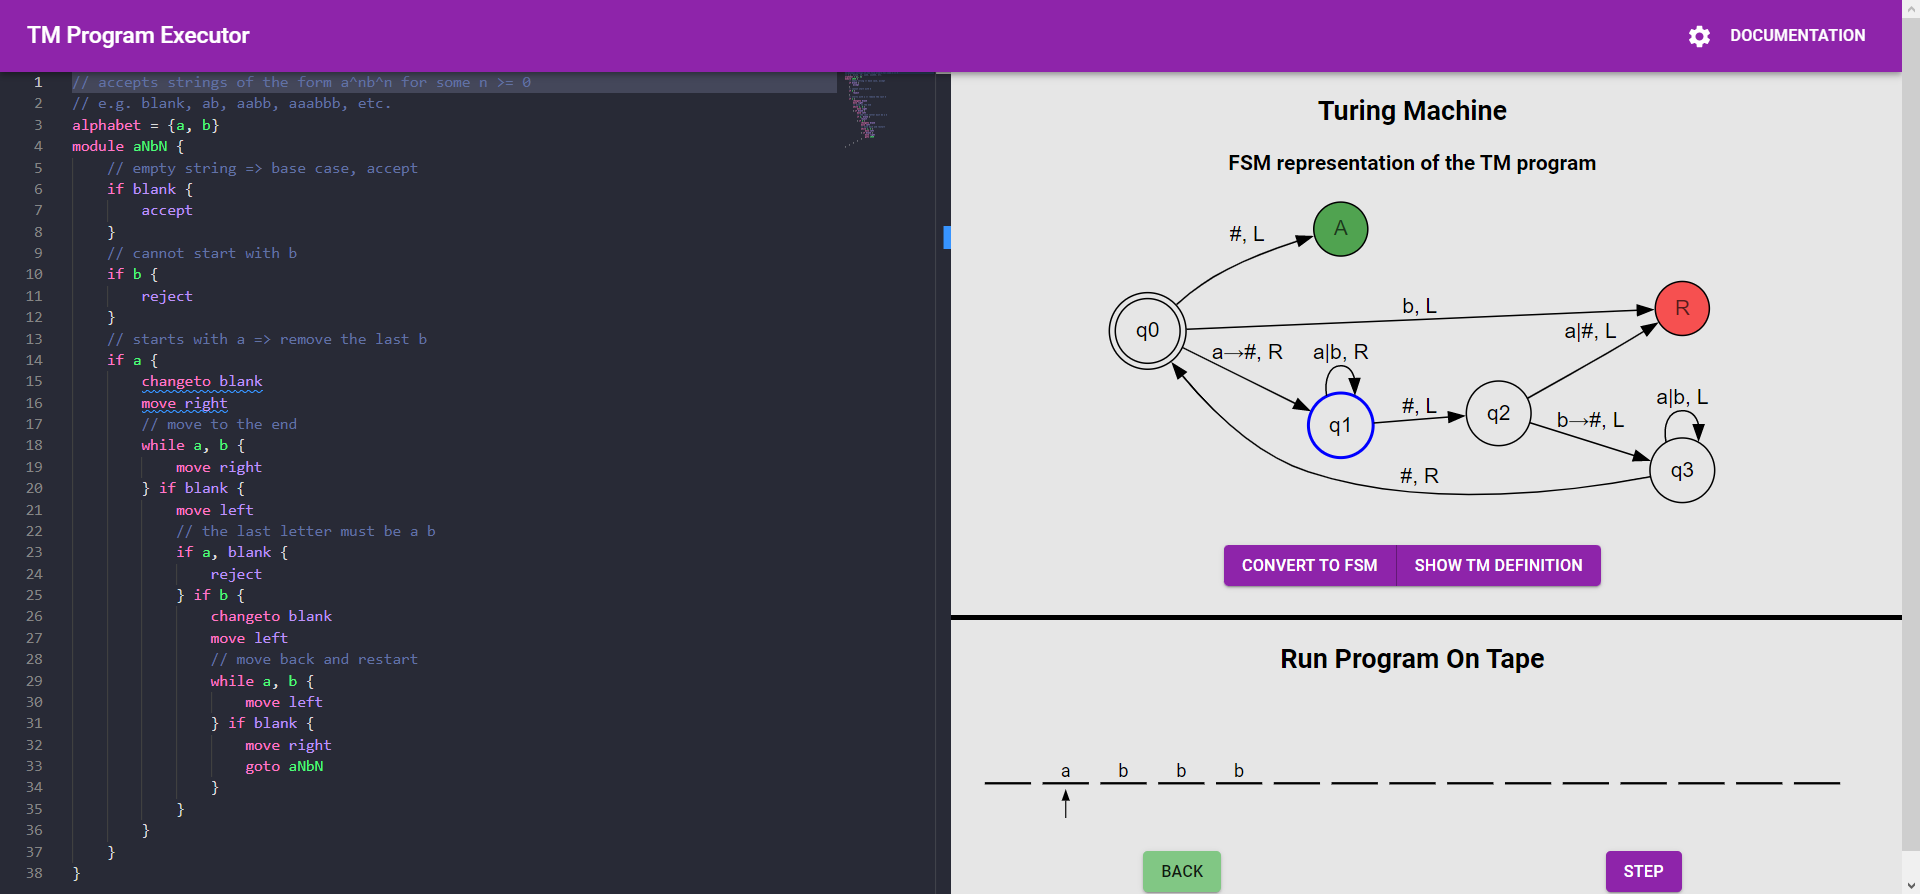
\includegraphics[scale=0.18]{images/Homepage execution start.png}
    \caption{The website homepage.}
    \label{fig:homepage_design}
\end{figure}

The user can input a program to the editor. If the program is valid, it can be compiled to a TM in two ways- it can either be converted to a FSM or to the definition version. The user can also execute the program on a tape after inputting a value. The step button performs one step in execution. 

The toolbar features a button to go to the documentation pages. There is also a button that allows the user to configure the page, e.g. fill the editor with some example code, change the editor theme, change font size, etc. 

\subsubsection{Documentation Pages}
The website has documentation pages that define both TMs and TML programs. In particular, the page:
\begin{itemize}
    \item gives the formal definition, 
    \item shows an example and 
    \item allows the user to execute the example on a tape.
\end{itemize}

\subsubsection{Error Pages}
For every language error, there is a dedicated page that:
\begin{itemize}
    \item describes the error informally;
    \item illustrates the error with an example program; and 
    \item presents a way to resolve the error.
\end{itemize}
There is also a general error page that lists all these errors.

The website makes use of \emph{Material Design}\footnote{\url{https://m3.material.io}}. The Material design provides common-purpose components, such as toolbars and icons. Moreover, Material design is quite widespread since all Google products make use of it. Hence, the user is expected to recognise these common constructs and should be able to easily interact with them. For instance, the user can recognise that a settings icon allows them to customise the website in some way. Furthermore, Material Design helps keep the website design responsive and consistent.

\subsection{TM Conversion}
The website supports live conversion of a TML program into a TM. The user can convert the TML program into both the FSM representation of a TM and its definition.

\begin{table}[htb]
    \centering
    \begin{tabular}{c|ccc}
        & $0$ & $1$ & $\#$ \\
        \hline
        $q_0$ & $(R, 0, q_0)$ & $(R, 1, q_0)$ & $(L, \#, q_1)$ \\
        $q_1$ & $(L, 0, q_A)$ & $(L, 1, q_R)$ & $(L, 1, q_R)$ 
    \end{tabular}
    \caption{A transition table.}
    \label{tbl:table_isDiv2}
\end{table}

The formal definition of the TM defines all the states and then presents the transitions in a table, such as the one in Table \ref{tbl:table_isDiv2}. In this example, the non-terminating states are $q_0$ and $q_1$, and the alphabet $\Sigma = \{0, 1\}$. Moreover, the transition table says that $\delta(q_0, 0) = (R, 0, q_0)$, meaning that, during execution:
\begin{itemize}
    \item the tapehead pointer moves to the \emph{right};
    \item the tapehead value stays $\emph{0}$; and 
    \item the current state remains $\emph{q}_\emph{0}$
\end{itemize}

\subsection{Tape Execution}
The user can input a valid string in the alphabet and execute the TML program on a tape. A valid string consists of letters in the alphabet and the blank symbol. The tape panel features 15 visible tape entries (positions for an input value). The tape panel animates the execution process in the tape entries, which involves:
\begin{itemize}
    \item changing the tapehead value; and
    \item moving the tape to the left or the right.
\end{itemize}
Note that a \textit{move} command moves the \textit{pointer}, not the tape. Hence, the command \texttt{move left} moves the tape to the \textit{right}; the tapehead position remains constant.

\begin{figure}[htb]
    \centering
    \begin{subfigure}{0.3\textwidth}
        \centering
        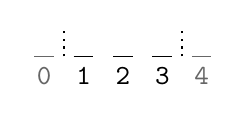
\begin{tikzpicture}
            \foreach \x in {0, 4} {
                \draw[opacity=0.6] (\x*0.5, 0) -- (\x*0.5+0.25, 0);
                \node[opacity=0.6] at (\x*0.5+0.125, -0.25) {\texttt{\x}};
            }
            \foreach \x in {1, 2, 3} {
                \draw (\x*0.5, 0) -- (\x*0.5+0.25, 0);
                \node at (\x*0.5+0.125, -0.25) {\texttt{\x}};
            }

            \draw[thick, dotted] (0.375, 0) -- (0.375, 0.35);
            \draw[thick, dotted] (1.875, 0) -- (1.875, 0.35);
        \end{tikzpicture}
        \caption{}
    \end{subfigure}
    \hfill
    \begin{subfigure}{0.3\textwidth}
        \centering
        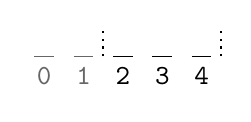
\begin{tikzpicture}
            \foreach \x in {0, 1} {
                \draw[opacity=0.6] (\x*0.5, 0) -- (\x*0.5+0.25, 0);
                \node[opacity=0.6] at (\x*0.5+0.125, -0.25) {\texttt{\x}};
            }
            \foreach \x in {2, 3, 4} {
                \draw (\x*0.5, 0) -- (\x*0.5+0.25, 0);
                \node at (\x*0.5+0.125, -0.25) {\texttt{\x}};
            }

            \draw[thick, dotted] (0.875, 0) -- (0.875, 0.35);
            \draw[thick, dotted] (2.375, 0) -- (2.375, 0.35);
        \end{tikzpicture}
        \caption{}
    \end{subfigure}
    \hfill
    \begin{subfigure}{0.3\textwidth}
        \centering
        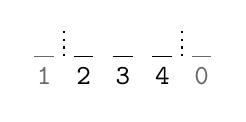
\begin{tikzpicture}
            \foreach \x[evaluate={int(mod(\x, 5))} as \y] in {5, 1} {
                \draw[opacity=0.6] (\x*0.5, 0) -- (\x*0.5+0.25, 0);
                \node[opacity=0.6] at (\x*0.5+0.125, -0.25) {\texttt{\y}};
            }

            \foreach \x in {2, 3, 4} {
                \draw (\x*0.5, 0) -- (\x*0.5+0.25, 0);
                \node at (\x*0.5+0.125, -0.25) {\texttt{\x}};
            }

            \draw[thick, dotted] (0.875, 0) -- (0.875, 0.35);
            \draw[thick, dotted] (2.375, 0) -- (2.375, 0.35);
        \end{tikzpicture}
        \caption{}
    \end{subfigure}
    \caption{The transition process for tape entries.}
    \label{fig:tape_movement}
\end{figure}

For the tape movement animation to look smooth, there are always 2 tape entries to either side of the tape. That way, if the tape gets moved left or right, there will be a tape entry to show. This is illustrated in Figure \ref{fig:tape_movement} (a)- the tape entries 0 and 4 are out of frame and therefore invisible. 

When the tape moves, there will be 2 tape entries on one side. For instance, if the tape moves to the left in Figure \ref{fig:tape_movement} (a), we get Figure \ref{fig:tape_movement} (b)- there are 2 invisible entries to the left. After the transition has completed, we move the most extreme tape entry to the other side. In the example, we move tape entry 0 to the right, leading to the tape state given in Figure \ref{fig:tape_movement} (c). At this point, we also change the tape value of entry 0 so that it matches the value at index 5. Since these changes are invisible, they take place instantly after the animation is complete.

\chapter{Implementation}
\section{Parser}

The parser was written in TypeScript. Although there are many frameworks that could have been used for lexical and syntactic analysis, these were not chosen. The main reason for this is that the parser was meant to be used within a website. In particular, it was expected that the parser became an node package manager (NPM) package. Moreover, TML is quite a simple language, making this task relatively easy and short.

\begin{figure}[htb]
    \centering
    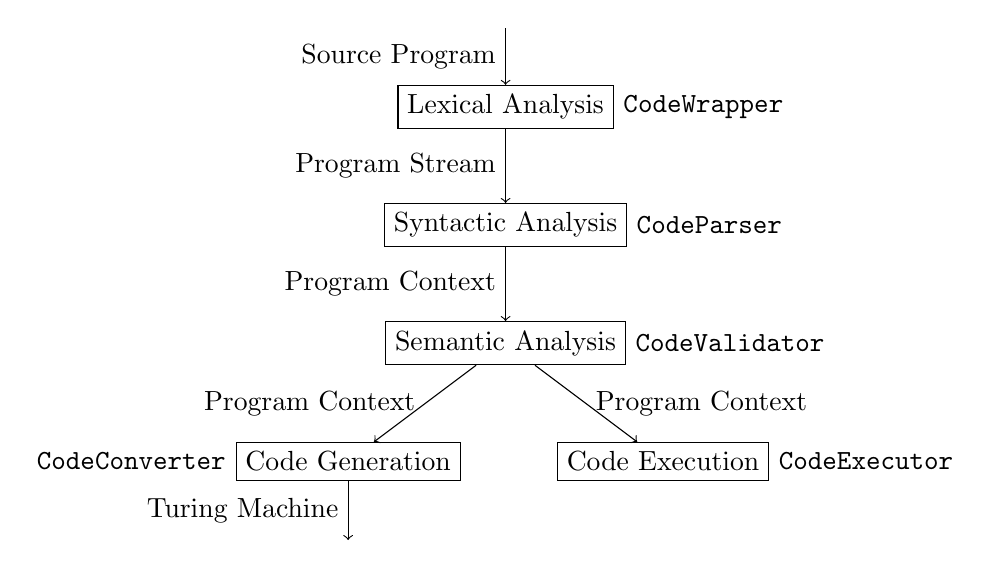
\begin{tikzpicture}
        \node[draw, label={0:\texttt{CodeWrapper}}] (CW) at (0, 0) {Lexical Analysis};
        \node[draw, label={0:\texttt{CodeParser}}] (CP) at (0, -1.5) {Syntactic Analysis};
        \node[draw, label={0:\texttt{CodeValidator}}] (CV) at (0, -3) {Semantic Analysis};
        \node[draw, label={180:\texttt{CodeConverter}}] (CC) at (-2, -4.5) {Code Generation};
        \node[draw, label={0:\texttt{CodeExecutor}}] (CE) at (2, -4.5) {Code Execution};

        \draw[->] (0, 1) -- node[left] {Source Program} (CW);
        \draw[->] (CW) -- node[left] {Program Stream} (CP);
        \draw[->] (CP) -- node[left] {Program Context} (CV);
        \draw[->] (CV) -- node[left] {Program Context} (CC);
        \draw[->] (CV) -- node[right] {Program Context} (CE);
        \draw[->] (CC) -- node[left] {Turing Machine} (-2, -5.5);
    \end{tikzpicture}
    \caption{The parsing process. The process is given inside the box. The class used to achieve the process is given in label, outside of the box. The flow of data is also shown.}
    \label{fig:parsing_process}
\end{figure}

The entire parsing process is summarised in Figure \ref{fig:parsing_process}.


\subsection{Lexical Analysis}

During lexical analysis, a stream of source code was produced. Although the source code was not enriched into tokens, the position of the code was tracked. This was to ensure that, in case of an error, the right section of code could be highlighted. This is done using the class \texttt{CodeWrapper}. 

To produce a stream of tokens, the iterator design pattern was used. The iterator design pattern allows us to get the current value from a collection in a way that abstracts the data structure (\cite{gamma1995design}). In particular, the pattern was used to abstract the string representation of the source code and return a single entry from the code at a time. 

\subsection{Syntactic Analysis}
\begin{figure}[htb]
    \centering
    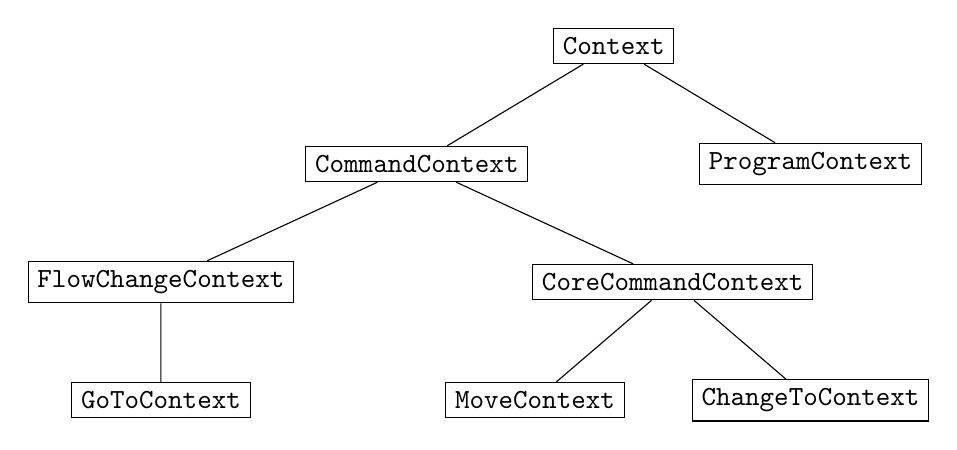
\begin{tikzpicture}[
        level 1/.style={sibling distance=5cm},
        level 2/.style={sibling distance=6.5cm},
        level 3/.style={sibling distance=3.5cm},
    ]
        \node[draw] {\texttt{Context}}
        child {
            node[draw] {\texttt{CommandContext}}
            child {
                node[draw] {\texttt{FlowChangeContext}}
                child {
                    node[draw] {\texttt{GoToContext}}
                }
            }
            child {
                node[draw] {\texttt{CoreCommandContext}}
                child {
                    node[draw] {\texttt{MoveContext}}
                }
                child {
                    node[draw] {\texttt{ChangeToContext}}
                }
            }
        }
        child {
            node[draw] {\texttt{ProgramContext}}
        };
    \end{tikzpicture}
    \caption{A snippet of the \texttt{Context} class hierarchy. All the non-leaf classes are abstract.}
    \label{fig:context_hierarchy}
\end{figure}

Next, the code is parsed. This is done using the class \texttt{CodeParser}. 

The result of the parsing is a \texttt{ProgramContext}, which represents the root of the AST. Subclasses of the \texttt{Context} class are used to represent different statements in the class, such as \texttt{MoveContext} for \textit{move} commands and \texttt{GoToContext} for \textit{goto} commands. A snippet of the class hierarchy for \texttt{Context} is shown in Figure \ref{fig:context_hierarchy}.

The parsing process results in the construction of the AST, such as the one in Figure \ref{fig:TML_AST}. To descend to a child, we make use of the instance fields. For instance, \texttt{ProgramContext} has the following fields:
\begin{itemize}
    \item \texttt{alphabet} for \texttt{AlphabetContext}; and
    \item \texttt{modules} for an array of \texttt{ModuleContext}.
\end{itemize}

The parser is recursive-descent and top-down in nature, as we can see in the \texttt{parseProgram} method below.
\begin{lstlisting}[language=TypeScript]
parseProgram() {
    var alphabet = parseAlphabet();
    
    var modules = [];
    while (code.moveNext()) {
        modules.add(parseModule());
    }
    
    return new ProgramContext(position, alphabet, modules);
}
\end{lstlisting}
Note that the code given above is simplified from the actual implementation.

If the program has syntax errors, then it will not be possible to produce an AST. For instance, the alphabet for the program might not been provided. This is detected by the parser since it makes use of predictive parsing. In particular, the parser looks at the next value and determines if it is legal; otherwise, it throws a \texttt{SyntaxError}.

\subsection{Semantic Analysis}
During semantic analysis, we traverse the AST using the \emph{visitor design pattern}. The visitor design pattern allows us to construct the same method for a class hierarchy without making changes to the classes (\cite{gamma1995design}). In particular, we want to create a method to validate each \texttt{Context}.

To allow for visitor design pattern, a concrete \texttt{Context} class implements the method \texttt{validate}. Each concrete class makes use of the right method from the \texttt{CodeValidator} class. We illustrate this with an example. Consider the following snippet of \texttt{GoToContext}.
\begin{lstlisting}[language=TypeScript]
class GoToContext extends FlowChangeContext {    
    identifier:string;
    
    validate(validator:CodeValidator):void {
        return validator.validateGoTo(this);
    }

    // ... other methods for goto context
}
\end{lstlisting}
    In that case, we can define the following method to `visit' a \textit{goto} statement and validate it.
\begin{lstlisting}[language=TypeScript]
class TypeValidator {
    validate(context:Context):void {
        return context.validate(this);
    }
    
    // validate that the goto identifier a module name
    validateGoTo(gotoContext:GoToContext):void {
        if (!moduleNames.contains(gotoContext.identifier)) {
            throw new CodeError("Undefined name- " + identifier);
        }
    }

    // ... other validator methods
}
\end{lstlisting}
To run the \texttt{CodeValidator}, we validate \texttt{ProgramContext}.

When traversing the AST, we typically want to aggregate the result or share the result with the parent. For this reason, we typically return a specific type of values within each visit method. 

In \texttt{CodeValidator}, we return \texttt{true} if a block has a flow command. This data is used in containers that have multiple blocks, such as a module. We throw an error if a non-final block has a flow command. Note that we always return \texttt{true}, e.g. even in \texttt{ProgramContext}, since the pattern must be followed by all the subclasses of \texttt{Context}. 

The advantage of using the visitor design pattern is that we have a way of traversing the AST without altering any of the \texttt{Context} classes; we can just construct a \texttt{Visitor} class. However, if we wanted to add another \texttt{Context} subclass, then we would need to amend all the \texttt{Visitor} classes. We expect the language to be pretty static, so this is perfectly fine in our case.


\subsection{TM Generation}
Next, we convert the AST into a TM. The TM is implemented in the class \texttt{TuringMachine} and mimics the definition of a TM.

We traverse the AST using the visitor design pattern. Initially, we define the TM and add relevant states and transitions during the traversal. The visitor methods return the label of the next state, if applicable to the context. This is defined in a very complex manner, depending on whether we have an \textit{if} or a \textit{while} command, or none at all.

\subsection{Code and TM Execution}
Finally, a validated program can be executed using \texttt{CodeExecutor}. This class follows the iterator design pattern. In particular, we can make use of the method \texttt{execute} to run one step in execution. This method returns \texttt{false} if and only if execution has not terminated. The steps of execution are defined precisely in the language specification, given in the appendix.

Unlike the previous two stages, code execution does not make use of the visitor design pattern. This is because we do not need to traverse the AST in one go to convert the program. Instead, it makes more sense to use the iterator design pattern- this supports execution one step at a time.

TM execution has also been implemented in the class \texttt{TMExecutor}. This also makes use of the iterator design pattern and supports execution one step at a time.

\section{Product}
Due to the complex nature of the website, it made use of many APIs.

At the start of the implementation, 3 frameworks were considered for the website:
% TODO: Source all 3 frameworks
\begin{itemize}
    \item the \emph{Webpack} framework- it has little overhead, allows for a lot of flexibility, but does not directly have components (such as toolbar and drawer) or support state management;
    \item the \emph{React} framework- it has a rich collection of components and supports state management directly;
    \item the \emph{Angular} framework- like React, it has a rich collection of components and supports state management.
\end{itemize}

% The React framework was chosen because it has a rich collection of components (such as a toolbar and a drawer) and has direct support for \emph{state management}. 
\emph{State management} was an important consideration when choosing the framework since the website tracks many states, such as the value of the editor and the current TM. Hence, it is particularly important that state management is readily supported by the framework. For this reason, webpack was not chosen.

Both React and Angular would have been equally good choices for the project. React was chosen as there are more APIs that readily integrate with React compared to Angular, includes some of the APIs used in this project. This is true since React is more widely used than Angular.
% TODO: Source
The React framework supports coding in either JavaScript or TypeScript. The project made use of the TypeScript version for type safety.

% The React framework makes use of components when rendering, which can be nested. This allows the website to be modularised. For instance, the homepage component was broken into 3 components- editor, TM and tape. These components can be further broken down into components, e.g. the TM component is composed of the FSM component and the definition component.

% Components also allow for reuse. For instance, the tape component makes use of 17 tape entry components that have the same behaviour. Moreover, the homepage and the documentation pages share the editor, tape and TM components.

The website made use of \emph{Material Design}. The components provided by the API are common-purpose, such as tables and drawers, and are easy to configure. Moreover, Material design is quite widespread since all Google products make use of it. 
% TODO: Source
Hence, the user is expected to recognise these common constructs and should be able to easily interact with them. For instance, the user can recognise that a settings icon allows them to customise the website in some way. Furthermore, Material Design helps keep the website consistent and responsive.

Screenshots of the website homepage, documentation and error pages are given in the appendix.

\subsection{Editor}

The editor feature was implemented using the \emph{monaco} API. The API was chosen since it integrates well with React and provides many features. The features include:
\begin{itemize}
    \item syntax highlighting with different priorities (e.g. an error gets an error priority while a code execution highlighting gets a low priority);
    \item the ability to easily set and get the current value; along with
    \item numerous customisations to the editor, such as as changing the font size, setting an editor theme and showing/hiding line numbers- these are all features that a user can configure in the website.
\end{itemize}
Moreover, the monaco editor was chosen since it has the same look as Visual Studio (VS) Code, and shares many functionalities with the IDE. A developer survey in 2022 found that VS Code is the most popular code editor among 70 000 developers.
% TODO: CITE using the reference in https://en.wikipedia.org/wiki/Visual_Studio_Code

\subsection{FSM Generation}
\begin{figure}[htb]
    \centering
    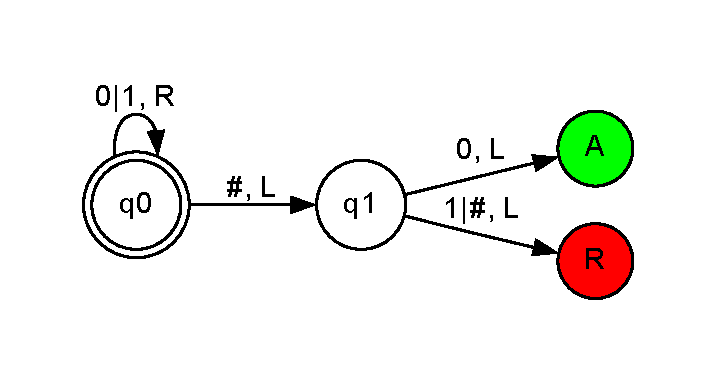
\includegraphics[scale=0.7]{images/graphviz_isDiv2.pdf}
    \caption{The graphviz rendering of the directed graph \texttt{isDiv2}.}
    \label{fig:graphviz_isDiv2}
\end{figure}

The FSM representation of the TM is created using the \emph{graphviz} framework. This makes use of the \emph{DOT} notation, which represents graphs in text by listing their nodes and edges. In particular, a graph in DOT notation is given below:
\begin{lstlisting}[language=DOT]
digraph isDiv2 {
    node [shape = "doublecircle"]; q0;
    node [shape = "circle"]; q1;
    node [style = "filled", fillcolor = "green"]; A;
    node [style = "filled", fillcolor = "red"]; R;
    q0 -> q0 [label = "0|1, R"];
    q0 -> q1 [label = "#, L"];
    q1 -> A [label = "0, L"];
    q1 -> R [label = "1|#, L"];
}
\end{lstlisting}
This graph represents the FSM representation of a TM. The keyword \texttt{digraph} implies that the graph is directed. The keyword \texttt{node} is used to create states. We use an arrow symbol (\texttt{->}) to construct edges between states.

Using the graphviz API, the graph in DOT notation can be rendered in the website- the result for the directed graph \texttt{isDiv2} is given in Figure \ref{fig:graphviz_isDiv2}. Note that the figure was produced with some extra formatting code that is not shown.

We convert a TM to DOT notation as follows:
\begin{itemize}
    \item we set the default formatting of a node to be a circle (similar to code in line 3 of the example);
    \item we list the initial state \texttt{q0}, the accept state \texttt{A} and the reject state \texttt{R}, with the right formatting (like in lines 2, 4 and 5); and 
    \item we then list all the edges and label it with the corresponding transition (like in lines 6-9).
\end{itemize}

The advantage of using the graphviz package is that it can produce a very well-formatted FSM. Initially, the graph was rendered by placing the states in order of its label, like in Figure \ref{tbl:table_isDiv2}. The user would be able to drag the states and hence achieve a more reasonable placement. However, there was time to make use of the graphviz package later in the project, and so the implementation was changed. Now, the user is unable to drag the states, but this should not be necessary as the states are already well-placed!

\subsection{TM Formal Definition Conversion}
% TODO: Mention that the definition is also given in a table representation (include a pic of that as well). Created using MathJax that takes in latex code and renders it as a SVG. Latex code follows the transition function of the TM.

The formal definition of a TM is constructed quite naturally by using the class \texttt{TuringMachine}- we can look at the \texttt{transition} function to find an object of type \texttt{TMChange}, which shows:
\begin{itemize}
    \item the next state value;
    \item the direction to move; and
    \item the value the tapehead value will become.
\end{itemize}
These 3 values are shown to the user in a table like the one in Figure \ref{tbl:table_isDiv2}.

The text in the table is constructed using the \emph{MathJax} framework. This framework compiles raw code in LaTeX and renders it as an SVG.

\subsection{Tape Execution}

The tape was implemented as a SVG elements. These were constructed using the \emph{d3} API. To illustrate tape execution, we make use of the animation subpackage in d3. In particular, this is used to move the tape left or right, and to change its value. 

During execution, we also highlight the current block being executed. Moreover, if the TM panel has been rendered, we highlight the current state and transition in the FSM representation. To keep track of these values, we execute the tape on both the TML program (using \texttt{CodeExecutor}) and its corresponding TM (using \texttt{TMExecutor}). We make use of the d3 API here as well to animate the change in current block/state.

\chapter{Evaluation} 
In the project, there were 2 aspects to evaluate- the TML and the website. Both aspects were evaluated continually through unit tests during production and tested using a user evaluation.

After the website had been completed, a user evaluation was conducted on 18 second year computing students. TMs are taught to students that have few years of programming experience, and for this reason second years were chosen. Note that they had little familiarity, if any, with Turing Machines and were introduced to both TMs and TML during the evaluation session. The aim of the evaluation was for them to get acquainted with the two concepts, and then to:
\begin{itemize}
    \item compare TMs and TML programs;
    \item understand whether writing a TML program would help in drawing a TM; and
    \item evaluate the website.
\end{itemize}
The evaluation session also served as a great opportunity to ask for any features to be added to the website and the language.

During the evaluation session, students were first introduced to TML programs. They were then expected to understand what language two mystery TML programs accept. This was done by checking whether the programs accepted some values, which should have helped them understand the way the program operates and decode the language it accepts. They were expected to use the website to help them follow the code and understand the steps in execution. Then, they were introduced to TMs, and expected to decode 2 TMs in a similar manner. Since the website can only execute TML programs, they were given TML programs for the TM. Note however that this did not defeat the purpose of testing TMs since:
\begin{itemize}
    \item most students found it easier to follow execution in TMs (a diagram) than TML (a program); and
    \item the programs given were complete TML programs, which are quite close to TMs.
\end{itemize}
Finally, they were asked to write some programs in the TML. Like in the previous sections, they were free to use the website to write the programs and test its correctness. The first few programs were quite similar to the code they had seen before. The remaining programs were somewhat more difficult, and for this reason they were optional. Nonetheless, many students attempted them and wrote impressive programs! The evaluation took about 50 minutes to be completed. The students were asked to fill out a worksheet with their answers. 

After they had completed the worksheet, they completed a survey to evaluate the language and the website. To avoid writing programs on paper, students were asked to copy their code from the final part of the worksheet to the survey. The results of the survey are discussed in detail in the next section. Both the worksheet and the survey are given in the appendix. 

\section{Evaluation Results}
\subsection{Parser and Language Evaluation}
The parser was continually tested during production to ensure correctness. This was achieved using unit testing. They were used to test all aspects of the parser, and were extensive. In fact, the unit tests had more than $95\%$ code coverage.

\begin{figure}
    \centering
    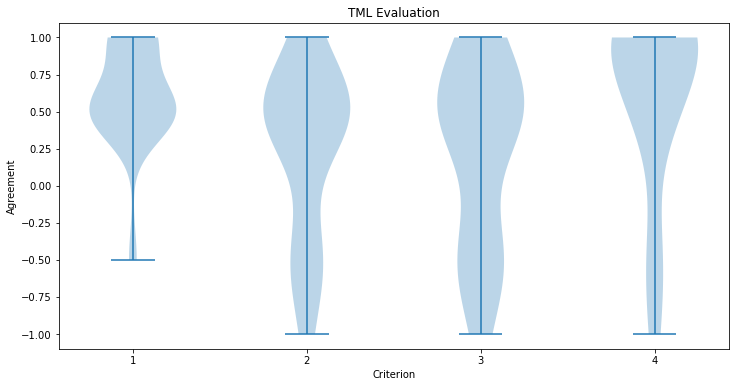
\includegraphics[scale=0.35]{data/tml-evaluation.png}
    \caption{A violin plot that summarises the results of the survey relating to the TML with respect to the 4 criteria. The agreement value refers to how much the user agrees to the statement: $-1$ is strongly disagree; $-0.5$ disagree; $0.5$ agree and $1$ strongly agree. The whiskers show the range of answers, e.g. nobody said they strongly disagreed with criterion 1. Moreover, the density is proportional to the number of participants answering the question with that value, e.g. most people answered criterion 1 with the value $0.5$ (agree).}
    \label{fig:tml-evaluation}
\end{figure}

During user evaluation, users were asked to evaluate the language in the following criteria:
\begin{enumerate}
    \item TML is easy to understand
    \item TML is easy to write programs in
    \item I was able to fix errors in my code using the error messages provided
    \item I was able to easily reason executing a program on a tape
\end{enumerate}
They were asked to rate how much they agreed with each statement, and the result is summarised for each criterion in Figure \ref{fig:tml-evaluation}. 

It is clear that most students found the language easy to understand. However, a smaller number of students believed that the language is easy to write programs in- the solutions to the worksheet illustrate that most students were able to correctly execute a program on a tape, and see whether it accepts a value, but found it harder to write (correct) programs. This is quite expected given that they were only exposed to the language for about an hour.

% the solutions to the worksheet illustrate that most students were able to correctly execute a program on a tape and see whether it accepts a value, but found it harder to describe all the types of values they accept. For instance, for a program that accepts values that are 3 mod 4, some students claimed that it accepts odd numbers. 

Most students found it easy to reason executing a program on a tape- they were able to run the code on the website and follow the code quite easily. Many found the error messages quite useful and it helped them write correct programs, but few disagreed with this. Some of the error messages could have been given more details, for example a missing case in a switch block did not identify what letter in the case was missing. Moreover, there was a minor bug in the position of the switch block (where it ended one line later than the correct position). The feedback from students helped identify these issues, and they were fixed in due time. 
% Also, some students also did not realise that they could hover over the error to see a message.

\begin{figure}
    \centering
    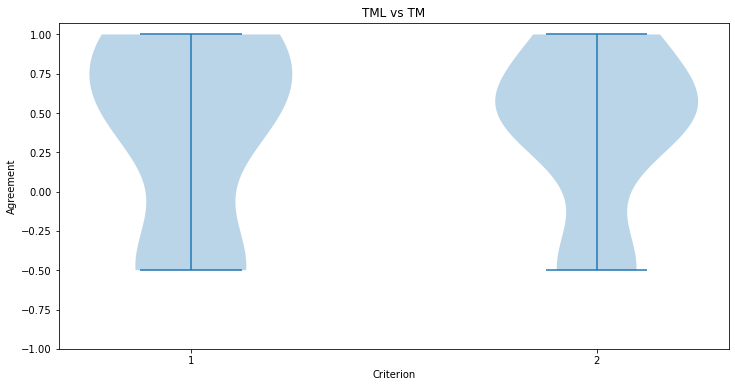
\includegraphics[scale=0.35]{data/tml-v-tm.png}
    \caption{A violin plot that summarises the results of the survey that compare TM and TML with respect to the 2 criteria.}
    \label{fig:tml-v-tm}
\end{figure}

The TML was then directly compared to TMs. In particular, students were asked to compare TMs and TML programs in the following criteria:
\begin{enumerate}
    \item I am more confident in writing a program in TML than drawing a TM
    \item I find it easier to reason what a TML program accepts than a TM
\end{enumerate}
The students were asked to rate how much they agreed with each statement, and the result is summarised for the two criteria in Figure \ref{fig:tml-v-tm}. 

Overall, students seem to be more comfortable with TML than TM. They were more confident writing a TML than drawing a TM- this is expected since they were not asked to draw a TM. However, it is surprising that many found it easier to reason a TML program than a TM. This is because many claimed that it is easier to follow a diagram than code. Nonetheless, the students might have found it easier to reason a TML program since the worksheet focuses much more on TML than TM.

% Students were also given an opportunity to make any general comments about the language and any features they would like to be added. Since the language has a similar structure to Java, a language that the students are quite familiar with, they found the language quite intuitive and easy to understand. Some mentioned that they struggled with the semantics of the language when writing code- as they weren't formally introduced to the syntax, this was expected. In particular, some students had changed the order of commands in a basic block, which meant that the code did not execute the way they had expected.

The students were then asked whether they would consider writing a TML program before drawing a TM. The response of this question is summarised in Figure \ref{fig:use-tml}. 

When drawing a TM for some algorithm, it is quite helpful to plan the machine beforehand. TML provides an opportunity where it is possible to reason in detail how the algorithm is meant to execute on a tape without considering the states and transitions in a TM. Moreover, it is quite easy to naturally convert a TML to a TM. I believe this is the main selling point of the language. The results clearly show that many would consider drawing it. The hesitation might result from the little experience that they had gotten.
% ; I would imagine that they would benefit writing a TML program, especially before drawing some complex TMs.

\begin{figure}
    \centering
    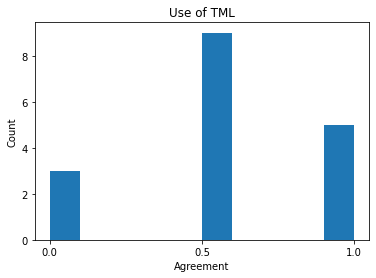
\includegraphics[scale=0.35]{data/use-tml.png}
    \caption{A histogram that summarises whether the users would consider writing a TML program before drawing a TM. 0 means no; 0.5 means maybe; and 1 means yes.}
    \label{fig:use-tml}
\end{figure}

\subsection{Website Evaluation}
Like with the language, the website was also continually tested during production for correctness. This was achieved through unit testing. Unlike the testing for language, this was however less successful due to the limits in mocking frameworks and time constraints. Nonetheless, the tests covered all the major parts of the website and ensured that all the functionalities implemented were correct.
% This was because of the use of frameworks in the website. They were mocked during testing, so all the functionalities they provide could not be tested completely.

\begin{figure}
    \centering
    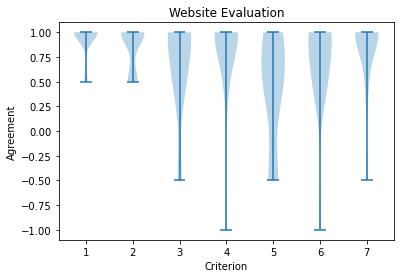
\includegraphics[scale=0.35]{data/website-evaluation.png}
    \caption{A violin plot that summarises the results of the survey relating to the website with respect to the 7 criteria.}
    \label{fig:website-evaluation}
\end{figure}

During the user evaluation, the students were expected to use the website to understand TMLs and TMs. For this reason, they were able to evaluate the website from their experience. In the survey, they were asked to evaluate the website in the following 7 criteria:
% Note that only the homepage could be evaluated; the documentation was not evaluated since I directly explained how the TML programs and TMs work. 
\begin{enumerate}
    \item The website is easy to follow
    \item The presentation of the website is intuitive
    \item There were no visible bugs in the website
    \item The website was fast
    \item The website feels complete
    \item The code execution was easy to follow
    \item The code editor was easy to use
\end{enumerate}
The results of the survey are summarised in Figure \ref{fig:website-evaluation}. 

It is evident that most found the website easy to follow and intuitive to use. Initially, there were a few bugs present in the website, e.g. the TM did not change to the latest version when tape execution began. However, in later sessions, most students believed that the website had few bugs. Most also found the website to be fast and complete. 

Some did not find code execution easy to follow- this was particularly the case with long programs where students had to scroll to find the currently executing block of code. Also, many found the code editor easy to use. There were some issues in using the code editor during the first session- the code cannot be edited while being executed, but there was no feedback to inform the user about this issue. In the later sessions, a warning pop-up was added to warn them of this issue and students were able to fix the issue easily.

% Following the user evaluation, it is clear that the TML has a lot of potential. Moreover, it might be easier to learn TML than TMs, although the result is not conclusive. I believe students will benefit from using TML, at least for planning how to draw TMs.
% TODO: Improve conclusion of evaluation

\section{Limitations to Evaluation}
Due to the time constraints of the project, there were some limitations to the evaluation, in user evaluation. The biggest limitation was the length of the evaluation session. It was hard to find a balance between a productive session and a short session. 
% Also, the questions were made quite simple since the intention was not to test the student's capability, but instead 
% In fact, the first evaluation session took considerably longer than an hour, after which I made substantial changes to the questions (i.e. made some easier and some others optional) to ensure that it fits within an hour!
For this reason, it was not possible to test the students' ability to draw TMs. Moreover, a significant portion of the question do not require the student to understand TMs or TML programs; they can just run the code on the website and get the answer. This was done to help the students grasp the language easily. When it came to describing the values that a program/TM accepted, it was clear that some had not understood the program. For instance, in a mystery program that accepts values that are 3 mod 4, some students claimed that the program accepts all odd numbers!
% This was deliberately not sufficient for some of the questions present, and showed that they had not fully understood the program/TM.
Moreover, although students were asked to write some TM programs, this could not be tested completely. In fact, the core questions only involved making minor changes to the programs they were given; it was only the optional questions that truly tested their ability to write TM programs and reason about them. 

% Finally, the sample size for the evaluation is quite small- only 18 people took part. So, any result from the evaluation is not conclusive.

% In terms of unit testing, the website has not been fully tested. This is because some of the functionalities of the website have not been fully mocked. In particular, the editor has not been mocked. This means that it is not possible to validate certain aspects of the editor, for example the user should not be able to edit the website during execution. By using a more sophisticated mocking technique, this should be possible to achieve, but this was not implemented in the project due to time constraints.

\chapter{Conclusion}

% Summarise the whole project for a lazy reader who didn't read the rest (e.g. a prize-awarding committee).
% -> Summarise briefly and fairly.
% ->  You should be addressing the general problem you introduced in the Introduction.        
% -> Include summary of concrete results (``the new compiler ran 2x faster'')

\section{Summary}
The project aimed to construct a language for Turing Machines and investigate whether it is easier to learn the concept the traditional manner or through programming. To allow for the comparison of the two techniques, the project as split into 3 construction phases:
\begin{itemize}
    \item defining the language;
    \item constructing a parser for the language;
    \item showcasing the parser in a website (the product).
\end{itemize}
The 3 phases were completed, after which there was an evaluation session aimed at comparing the teaching of Turing Machines using diagrams and programs.

The evaluation showed that the language is somewhat easier to understand and learn than the diagrammatic approach. However, due to the limited nature of the evaluation and the previous programming experience of the students, this result might not hold in general. This could likely be improved by adding some syntactic sugar to the language so that it abstracts further the details of Turing Machines.

\section{Reflection}
This project was quite an enjoyable experience for me. I was very happy to work on a self-defined project and that gave me a lot of motivation to work on it! It was also exciting connecting programming languages and Turing machines, and I found that quite exciting! This project has also taught me a lot about web development, in particular the React framework!

I do feel that due to the time constraints, I was not able to develop the language and the product completely. There are many extensions that I would have liked to add, as listed in future work. Nonetheless, I plan to work on adding these extensions during the summer!

\section{Future Work}

There are many additions that can be made to the language and the product in future. Some of these were discovered during production, and some as part of the user evaluation.

\subsection{Language}
Although the language is equivalent to TMs, and has a few features that resemble a traditional PL, it is still quite low-level. There are many common paradigms that can be added to the language. These include:
\begin{enumerate}
    \item the ability to traverse to the end (or the start) of the tape string in one command, e.g. \texttt{move end}; 
    \item an \textit{else} block (an \textit{if} block for the remaining letters); and
    \item the ability for modules to be parameterised with respect to letters.
\end{enumerate}
We illustrate these issues with the following program:
\lstinputlisting[language=TML]{code/fut_work_tml.txt}

The first feature is a very common feature found in program- many programs involving some check on the final character. For example, in the program above, we are traversing to the end twice- at lines 5-9 and 17-21. Hence, I believe this would be a highly beneficial feature to add.

The second point is also somewhat common and was suggested in the survey. At many points during execution, we want to do something for a single letter and something different for the other letters. For instance, in the example above, at lines 10-13, we want the program to accept the string if and only if the letter is a \texttt{b}. If the alphabet was longer, this would be quite inefficient. Also, another point that was raised during the survey was that the language only makes use of pattern-matching, and could be more flexible. So, this would be a great feature to extend the language. 

The final feature is quite interesting. There are many programs where the modules are very similar and only differ in some letters. For example, the program above has 2 essentially mirrored blocks at lines 4-16 and 16-28. In particular, the only difference in these lines of code is at lines 10/12 and 22/24, where the letters \texttt{a} and \texttt{b} are the other way round. Hence, I believe that adding this feature would make many programs in TML shorter and less repetitive! Moreover, this would make the language further resemble a traditional PL.

% Finally, there is an open question about the language- the ability to convert a TM into a `good' TML program. Currently, the proof of equivalence makes use of an algorithm to convert a valid TML program to a complete TML program, but not vice versa. Complete TML programs can be thought of as another representation for TMs, and so add no further benefit to the language. It is the ability to nest blocks within \textit{if} commands that really makes the language rich and different to TMs. For this reason, I believe it would be a good idea to devise an algorithm to convert a TM (or a complete TML program) to a nested TML program.

% One way to do so would be to achieve maximum nesting by replacing \texttt{goto} commands with the actual module, however this is not optimal- there would be a lot of duplicate code present. Instead, it might be a good idea to only replace modules that are only called once, and to keep modules that are called multiple times separate. The main benefit of this is that complete TML programs are essentially another representation of TMs and quite distant from TML programs. I believe valid, non-complete

 \subsection{Product}
There are many possible improvements to the website. These are some of the features that can be added:
\begin{itemize}
    \item support for direct execution of a TM;
    \item a play button on the tape section to execute long programs on long tapes without pressing the step button many times;
    \item the ability to collapse the panels; and
    \item the ability to customise the number of tape entries shown so that it is easier to follow code execution on long strings.
\end{itemize}
All of these are great features that could be added to the website and would make it easier to use!

We could also improve the website by making the TM panel more responsive. The FSM is currently being produced using the graphviz framework. The resulting SVG has hard-coded dimensions. This makes it hard to make the panel responsive. It is not completely possible to make the graph fixed; only the maximum size of the SVG can be specified. Moreover, the constraints are not taken into consideration when the API produces the FSM. This means that for complex TM, the states are quite small and hard to see. This makes it hard to follow the execution process. To fix this, we could add one of the following features:
\begin{itemize}
    \item the FSM might produced as it currently is, but the user can zoom in and drag the FSM panel; or
    \item the FSM might be produced so that the states always have the same size, but the user can scroll the panel. 
\end{itemize}
  
\begin{appendices}
\chapter{TML Specification}

In this chapter, we will define the syntax of the Turing Machine Language starting with an example. We next analyse the syntax and define execution of a valid TML program on a tape in a similar manner to the execution of a TM.

Consider the following TML program.
\lstinputlisting[language=TML]{code/isDiv2.txt}
A program in TML will be used to execute on a tape, so the syntax used guides us in executing the program on a tape. We will see that later. For now, we consider the rules of the TML program:
\begin{itemize}
    \item A valid TML \emph{program} is composed of the \emph{alphabet}, followed by one or more \emph{modules}. In the example above, the alphabet of the program is $\{0, 1\}$, and the program has a single module called \texttt{isEven}.
    \item A module contains one or more \emph{blocks} (a specific sequence of commands). There are two types of blocks- \emph{basic blocks} and \emph{switch blocks}.
    \item A basic block consists of \emph{basic commands} (\textit{changeto}, \textit{move} or \textit{flow} command). A basic block consists of at least one basic command, but it is not necessary for a basic block to be composed of all the basic commands. If multiple commands are present in a basic block, they must be in the following order- \textit{changeto}, \textit{move} and \textit{flow} command. In the program above, there is are many basic blocks, e.g. at lines 4, 6, 8-9 and 11-12. We do not say that line 8 is a basic block by itself; we want the basic block to be as long as possible.
    \item A \emph{switch block} consists of cases (\textit{if} or \textit{while} commands), each of which corresponds to one or more letters. A switch block must contain precisely one case for each of the letter in the alphabet, including the \texttt{blank} letter. The first block within a case block cannot be another switch block. In the program above, there is a switch block at lines 3-14 and a nested switch block at lines 7-13.
    \item The body of an \textit{if} command can be composed of multiple blocks. These blocks can be both basic blocks and switch blocks. We can see this at lines 5-13; the \textit{if} block has a basic block at line 6 and then a switch block.
    \item The body of a \textit{while} command must be composed of a single basic block. The basic block cannot have a \textit{flow} command. This is because when we execute a \textit{while} block, the next block to run is the switch block it is in; we cannot accept, reject or go to another module.
    \item A switch block must be the final block present; it cannot be followed by a basic block.
\end{itemize}
% The EBNF for the TML and examples of syntax errors are given in the appendix. 

The EBNF of the TML is given below:
\begin{align*}
    \textit{program} &= \textit{alphabet} \ \textit{module}^+ \\
    \textit{alphabet} &= \texttt{alphabet} \ \texttt{=} \ \texttt{\{} \ \textit{seq-val} \ \texttt{\}} \\
    \textit{module} &= \texttt{module} \ \textit{id} \ \texttt{\{} \ \textit{block}^+ \ \texttt{\}} \\
    \textit{block} &= \textit{basic-block} \ | \ \textit{switch-block} \\
    \textit{switch-block} &= \textit{case-block}^+ \\
    \textit{case-block} &= \textit{if-block} \ | \ \textit{while-block} \\
    \textit{if-block} &= \texttt{if} \ \textit{seq-val} \ \texttt{\{} \textit{block}^+ \texttt{\}} \\
    \textit{while-block} &= \texttt{while} \ \textit{seq-val} \ \texttt{\{} \ \textit{core-com}^+ \ \texttt{\}} \\
    \textit{basic-block} &= (\textit{core-com} \ | \ \textit{flow-com})^+ \\
    \textit{core-com} &= \texttt{move} \ \textit{direction} \ | \ \texttt{changeto} \ \textit{value} \\
    \textit{flow-com} &= \texttt{goto} \ \textit{id} \ | \ \textit{terminate} \\
    \textit{terminate} &= \texttt{reject} \ | \ \texttt{accept} \\
    \textit{direction} &= \texttt{left} \ | \ \texttt{right} \\
    \textit{seq-val} &= (\textit{value} \texttt{,})^* \ \textit{value} \\
    \textit{value} &= \texttt{blank} \ | \ \texttt{a} \ | \ \texttt{b} \ | \ \texttt{c} \ | \ \dots \ | \ \texttt{z} \ | \ \texttt{0} \ | \ \texttt{1} \ | \ \dots \ | \ \texttt{9} \\
    \textit{id} &= (\texttt{a} \ | \ \texttt{b} \ | \ \texttt{c} \ | \ \dots \ | \ \texttt{z} \ | \ \texttt{A} \ | \ \texttt{B} \ | \ \texttt{C} \ | \ \dots \ | \ \texttt{Z})^+
\end{align*}

We will now consider how to execute a tape on a valid TML program. Let $P$ be a TML program with alphabet $\Sigma$ and let $T$ be a tape on $\Sigma$. We execute $P$ on $T$ inductively, as follows:
\begin{itemize}
    \item At any point during execution, we maintain 3 objects- a tape on $\Sigma$, a block of $P$ and the tapehead index. 
    \item At the start, the tape is $T$; the tapehead index is $0$; and the block is the first block in the first module in $P$. 
    \item At some point during the execution, assume that we have the tape $S$, tapehead index $j$, with tapehead value $T(j) = t$, and a block $b$. We define the next triple as follows:
    \begin{itemize}
        \item if $b$ is a switch block, we take the first block from the case corresponding to the tapehead value- because the program is valid, this is a basic block; we will now refer to this block as $b$.
        \item if $b$ has a \textit{changeto} \texttt{val} command, the next tape $T'$ is given by 
        \[T'(x) = \begin{cases}
            \texttt{val} & x = i \\
            T(x) & \text{otherwise}.
        \end{cases}\]
        If the \textit{changeto} command is missing, then the tapehead $T' = T$.
        \item if $b$ has a \textit{move} \texttt{dir} command, the next tapehead index is given by:
        \[i' = \begin{cases}
            i+1 & \texttt{dir} = \texttt{right} \\
            i-1 & \texttt{dir} = \texttt{left}.
        \end{cases}\]
        If the \textit{move} command is missing, then $i' = i-1$.
        \item we either terminate or determine the next block $b'$ to execute (in decreasing precedence):
        \begin{itemize}
            \item if the block is the body of a while case block, then the next block $b' = b$, i.e. we execute this switch block again (not necessarily the same case block);
            \item if the block contains a terminating \textit{flow} command, execution is terminated and we return the terminated state (\texttt{accept} or \texttt{reject});
            \item if the block contains a \textit{goto} \texttt{mod} command, then $b'$ is the first block of the module \texttt{mod};
            \item if the block is not the final block in the current module, then $b'$ is next block in this module;
            \item otherwise, execution is terminated and we return the state \texttt{reject}.
        \end{itemize}
    \end{itemize}
    If execution is not terminated, execution continues with the next triplet.
\end{itemize}

We now illustrate the execution process. So, consider the following TML program:
\lstinputlisting[language=TML]{code/palindrome.txt}
We will execute the program on the following tape.
\begin{figure}[H]
    \centering
    \begin{tikzpicture}
        \draw[thick] (-0.25, 0) -- (0, 0);
        \foreach \x[count=\i] in {a, b, a} {
            \draw[thick] (\i*0.5-0.25, 0) -- (\i*0.5, 0);
            \node at (\i*0.5-0.125, 0.3) {\texttt{\x}};
        }
        \draw[thick] (1.75, 0) -- (2, 0);

        \draw[->, thick] (0.375, -0.5) -- (0.375, -0.1);
    \end{tikzpicture}
\end{figure}
\noindent The arrow points at the tapehead value. We first execute the first block in the module \texttt{palindrome}. Since the tapehead value is \texttt{a}, we execute the basic block at lines 5-20. So, we change the tapehead value to \texttt{blank}, and the tapehead moves to the right by one step. Since this is an \textit{if}-block, without a flow command, and there is a block following this one, the next block to be executed is the switch block at lines 8-19. Now, the current tape is the following.
\begin{figure}[H]
    \centering
    \begin{tikzpicture}
        \draw[thick] (-0.25, 0) -- (0, 0);
        \foreach \x[count=\i] in {b, a} {
            \draw[thick] (\i*0.5-0.25, 0) -- (\i*0.5, 0);
            \node at (\i*0.5-0.125, 0.3) {\texttt{\x}};
        }
        \draw[thick] (1.25, 0) -- (1.5, 0);

        \draw[->, thick] (0.375, -0.5) -- (0.375, -0.1);
    \end{tikzpicture}
\end{figure}
\noindent The current block is a switch block. The tapehead value is \texttt{b}, so we are at the \textit{while} command at line 9. The basic block here only contains a \textit{move} command. So, we leave the tape as is, and the tapehead moves to the right once. This is a \textit{while} command, so the next block to execute is still this switch block. The current tape state is the following.
\begin{figure}[H]
    \centering
    \begin{tikzpicture}
        \draw[thick] (-0.25, 0) -- (0, 0);
        \foreach \x[count=\i] in {b, a} {
            \draw[thick] (\i*0.5-0.25, 0) -- (\i*0.5, 0);
            \node at (\i*0.5-0.125, 0.3) {\texttt{\x}};
        }
        \draw[thick] (1.25, 0) -- (1.5, 0);

        \draw[->, thick] (0.875, -0.5) -- (0.875, -0.1);
    \end{tikzpicture}
\end{figure}
\noindent The current block is still a switch block. The tapehead value is \texttt{a}, so we execute the same \textit{while} command at line 9. Moreover, the next block to execute is still the switch block. Now, the current tape state is the following.
\begin{figure}[H]
    \centering
    \begin{tikzpicture}
        \draw[thick] (-0.25, 0) -- (0, 0);
        \foreach \x[count=\i] in {b, a} {
            \draw[thick] (\i*0.5-0.25, 0) -- (\i*0.5, 0);
            \node at (\i*0.5-0.125, 0.3) {\texttt{\x}};
        }
        \draw[thick] (1.25, 0) -- (1.5, 0);

        \draw[->, thick] (1.375, -0.5) -- (1.375, -0.1);
    \end{tikzpicture}
\end{figure}
\noindent For the third time, we are executing the same switch block. Now, however, the tapehead value is \texttt{blank}, so we execute the first block of the \textit{if} command at line 5, i.e. we move to the left. Since this is an \textit{if} command and this is not the last block in the if command, the next block to execute is the switch block at lines 12-18.
\begin{figure}[H]
    \centering
    \begin{tikzpicture}
        \draw[thick] (-0.25, 0) -- (0, 0);
        \foreach \x[count=\i] in {b, a} {
            \draw[thick] (\i*0.5-0.25, 0) -- (\i*0.5, 0);
            \node at (\i*0.5-0.125, 0.3) {\texttt{\x}};
        }
        \draw[thick] (1.25, 0) -- (1.5, 0);

        \draw[->, thick] (0.875, -0.5) -- (0.875, -0.1);
    \end{tikzpicture}
\end{figure}
\noindent Now, the current block is a switch block. The tapehead value is \texttt{a}, so we take the basic block at lines 12-16. The value of the tapehead becomes \texttt{blank}, and moves to the left. The next block to execute is the switch block in \texttt{restart}.
\begin{figure}[H]
    \centering
    \begin{tikzpicture}
        \draw[thick] (-0.25, 0) -- (0, 0);
        \foreach \x[count=\i] in {b} {
            \draw[thick] (\i*0.5-0.25, 0) -- (\i*0.5, 0);
            \node at (\i*0.5-0.125, 0.3) {\texttt{\x}};
        }
        \draw[thick] (0.75, 0) -- (1, 0);

        \draw[->, thick] (0.375, -0.5) -- (0.375, -0.1);
    \end{tikzpicture}
\end{figure}
\noindent Since the current tapehead value is \texttt{b}, we execute the basic block at line 39. So, we move to the left, and the tape is left as is. Moreover, since this is a while block, the next block to execute is still the switch block.
\begin{figure}[H]
    \centering
    \begin{tikzpicture}
        \draw[thick] (-0.25, 0) -- (0, 0);
        \foreach \x[count=\i] in {b} {
            \draw[thick] (\i*0.5-0.25, 0) -- (\i*0.5, 0);
            \node at (\i*0.5-0.125, 0.3) {\texttt{\x}};
        }
        \draw[thick] (0.75, 0) -- (1, 0);

        \draw[->, thick] (-0.125, -0.5) -- (-0.125, -0.1);
    \end{tikzpicture}
\end{figure}
\noindent Since the current tapehead state is \texttt{blank}, we execute the basic block at lines 40-43. So, we move to the left, and the tape is left as is. The next block to execute is the switch block at \texttt{palindrome}.
\begin{figure}[H]
    \centering
    \begin{tikzpicture}
        \draw[thick] (-0.25, 0) -- (0, 0);
        \foreach \x[count=\i] in {b} {
            \draw[thick] (\i*0.5-0.25, 0) -- (\i*0.5, 0);
            \node at (\i*0.5-0.125, 0.3) {\texttt{\x}};
        }
        \draw[thick] (0.75, 0) -- (1, 0);

        \draw[->, thick] (0.375, -0.5) -- (0.375, -0.1);
    \end{tikzpicture}
\end{figure}
\noindent Since the current tapehead state is \texttt{b}, we execute the basic block at lines 21-22. So, we change the tapehead value to \texttt{blank}, move to the right. This is a while block, so the next block to be executed is still the switch block.
\begin{figure}[H]
    \centering
    \begin{tikzpicture}
        \draw[thick] (-0.25, 0) -- (0, 0);
        \draw[thick] (0.25, 0) -- (0.5, 0);
        \draw[thick] (0.75, 0) -- (1, 0);

        \draw[->, thick] (0.875, -0.5) -- (0.875, -0.1);
    \end{tikzpicture}
\end{figure}
\noindent At this point, the tapehead index moves between the blank values as we move to the basic block at line 3. Then, the execution terminates and we accept the tape.

\chapter{Proof of Equivalence}
In this chapter, we give a proof of equivalence between TMs and TML programs. This is done in many steps that involve:
\begin{itemize}
    \item proving that a TM can be converted to a complete TML program with the same behaviour;
    \item proving that a complete TML program can be converted to a TM with the same behaviour; and
    \item proving that a valid TML program can be converted to a complete TML program with the same behaviour.
\end{itemize}

\section{Complete TML Programs}
When we defined execution of a valid TML program on a tape above, we said that a basic block need not have all 3 types of commands (\textit{changeto}, \textit{move} and a \textit{flow} command), but in the execution above, we have established some `default' ways in which a program gets executed. In particular,
\begin{itemize}
    \item if the \textit{changeto} command is missing, we do not change the value of the tape;
    \item if the \textit{move} command is missing, we move left;
    \item if the \textit{flow} command is missing, we can establish what to do using the rules described above- this is a bit more complicated than the two commands above.
\end{itemize}
Nonetheless, it is possible to include these `default' commands to give a \emph{complete} version of the program. This is what we will establish in this section. 

Consider the following complete program.
\begin{lstlisting}[language=TML]
alphabet = {"0", "1"}
module isOdd {
    // move to the end
    while 0 {
        changeto 0
        move right
    } while 1 {
        changeto 1
        move right
    } if blank {
        changeto blank
        move left
        goto isOddCheck
    }
}
module isOddCheck {
    // accept if and only if the value is 1
    if 0, blank {
        changeto 0
        move left
        reject
    } if 1 {
        changeto blank
        move left
        accept
    }
}
\end{lstlisting}
Now, we consider the rules that a complete TML program obeys:
\begin{itemize}
    \item A basic block in a complete program has all the necessary commands- if the basic block is inside \textit{while} case, it has a \textit{changeto} command and a \textit{move} command; otherwise, it also has a \textit{flow} command.
    \item A module in a complete program is composed of a single switch block.
\end{itemize}

% By adding the `default' values for the \textit{changeto} and the \textit{move} command, we can partly complete a valid TML program. We can further break 
We will now construct a complete TML program for a valid TML program.
\begin{enumerate}
    \item We first break each module into smaller modules so that every module has just one basic/switch block- we add a \textit{goto} command to the next module if it appeared just below this block.
    \item Then, we can convert each basic block to a switch block by just adding a single case that applies to each letter in the alphabet.
    \item Finally, we add the default values to each basic block to get a complete TML program.
\end{enumerate}
This way, we can associate every block in the valid program with a corresponding block in the complete program. The complete version is always a switch block and might have more commands than the original block, but it still has all the commands present in the original block. 

We now illustrate this process with an example. Assume we first have the following program.
\begin{lstlisting}[language=TML]
alphabet = {"a", "b"}
module simpleProgram {
    changeto b
    move left
    move right
    accept
}
\end{lstlisting}
After applying step 1 of completion, we get the following program.
\begin{lstlisting}[language=TML]
alphabet = {"a", "b"}
module simple1 {
    changeto b
    move left
    goto simple2
}
module simple2 {
    move right
    accept
}
\end{lstlisting}
After applying step 2, we have the following program.
\begin{lstlisting}[language=TML]
alphabet = {"a", "b"}
module simple1 {
    if a, b, blank {
        changeto b
        move left
        goto simple2
    }
}
module simple2 {
    if a, b, blank {
        move right
        accept
    }
}
\end{lstlisting}
Finally, after applying step 3, we get the following program:
\begin{lstlisting}[language=TML]
alphabet = {"a", "b"}
module simple1 {
    if a {
        changeto b
        move left
        goto simple2
    } if b {
        changeto b
        move left
        goto simple2
    } if blank {
        changeto b
        move left
        goto simple2
    }
}
module simple2 {
    if a {
        changeto a
        move right
        accept
    } if b {
        changeto b
        move right
        accept
    } if blank {
        move right
        accept
    }
}
\end{lstlisting}
This program obeys the definition of a complete program.

\begin{theorem} \label{thm:complete_TM}
    Let $P$ be a valid TML program. Then, $P$ and its completion $P^+$ execute on every valid tape $T$ in the same way. That is,
    \begin{itemize}
        \item for every valid index $n$, if we have tape $T_n$, tapehead index $i_n$ and module $m_n$ with executing block $b_n$ for the TM program $P$, and we have tape $S_n$, tapehead index $j_n$ and module $t_n$, then $T_n = S_n$, $i_n = j_n$, and $t_n$ is the corresponding complete module block of $b_n$;
        \item $P$ terminates execution on $T$ if and only if $P^+$ terminates execution on $T$, with the same final status (\texttt{accept} or \texttt{reject}).
    \end{itemize}
\end{theorem}
\begin{proof}
    We prove this by induction on the execution step (of the tape). 
    \begin{itemize}
        \item At the start, we have the same tape $T$ for both $P$ and $P^+$, with tapehead index 0. Moreover, the corresponding (completed) module of the first block in the first module of $P$ is the first module of $P$. So, the result is true if $n = 0$. 
        \item Now, assume that the result is true for some integer $n$, where the block $b_n$ in the TML program $P$ does not end with a terminating \textit{flow} command. Let $\sigma_n$ be the letter at index $i_n = j_n$ on the tape $S_n = T_n$.
        \begin{itemize}
            \item If the \textit{changeto} command is missing in $b_n$ for $\sigma_n$, then the next tape $T_{n+1} = T_n$. In the complete module $m_n$, the case for $\sigma_n$ will have the command \texttt{changeto} $\sigma_n$. So, the next tape is given by:
            \[S_{n+1}(x) = \begin{cases}
                S_n(x) & x \neq j_n \\
                \sigma_n & \text{otherwise}
            \end{cases}.\]
            Therefore, we have $S_{n+1} = S_n$ as well. So, $T_{n+1} = S_{n+1}$. Otherwise, we have the same \textit{changeto} command in the two blocks, in which case $T_{n+1} = S_{n+1}$ as well.
            
            \item If the \textit{move} command is missing in $b_n$ for $\sigma_n$, then the next tapehead index $i_{n+1} = i_n - 1$. In the complete module $m_n$, the case for $\sigma_n$ will have the command \texttt{move left}, so we also have $j_{n+1} = j_n - 1$. Applying the inductive hypothesis, we have $i_{n+1} = j_{n+1}$. Otherwise, we have the same \textit{move} command, meaning that $i_{n+1} = j_{n+1}$ as well.
            
            \item We now consider the next block $b_{n+1}$:
            \begin{itemize}
                \item If the block $b_n$ is a \textit{switch} block with a \textit{while} case for $\sigma_n$, then this is still true in the module $m_n$. So, the next block to be executed in $P$ is $b_n$, and the next module to be executed in $P^+$ is $m_n$. In that case, the corresponding module of the block $b_{n+1} = b_n$ is still $m_{n+1} = m_n$.
    
                \item Instead, if the block $b_n$ has no \textit{flow} command for $\sigma_n$, and is not the last block, then the next block to execute is the block just below $b_n$, referred as $b_{n+1}$. By the definition of $P^+$, we find that the case block in the module $m_n$ has a \textit{goto} command, going to the module $m_{n+1}$ which corresponds to the block $b_{n+1}$. 
            
                \item Now, if the \textit{flow} command is missing for $\sigma_n$ and this is the last block, then execution is terminated with the status \texttt{reject} for the program $P$. In that case, the case for $\sigma_n$ in the module $m_n$ has the \texttt{reject} command present, so the same happens for $P^+$ as well. 
            
                \item Otherwise, both $P$ and $P^+$ have the same flow command, meaning that there is either correspondence between the next module to be executed, or both the program terminate with the same status. 
            \end{itemize}
        \end{itemize}
    \end{itemize}
    In that case, $P$ and $P^+$ execute on $T$ the same way by induction.
\end{proof}

Because of the equivalence between valid and complete programs, we will assume that every valid program is complete from now on.

\section{Equivalence of TMs and TMLs}
In this section, we will show that there is an equivalence between TMs and valid (complete) TML programs. We will first construct a valid TML program for a TM and then show that it has the same behaviour as the TM. Later, we will construct a TM for a complete TML program, and show the equivalence in this case as well.

We will first illustrate how to convert a TM to a (complete) TML program. So, consider the following TM:
Consider the following TM:
\begin{figure}[H]
    \centering
    \begin{tikzpicture}
        \node[state, accepting] (q1) at (2.5, 0) {$q_1$};
        \node[state, fill=green, opacity=0.6] (A) at (5, -1) {$A$};
        \node[state, fill=red, opacity=0.6] (R) at (5, 1) {$R$};

        \draw[->] (q1) edge[loop above] node[above] {$1, R$} (q1);
        \draw[->] (q1) -- node[below, rotate=-20] {$0, R$} (A);
        \draw[->] (q1) -- node[above, rotate=20] {$\#, R$} (R);
    \end{tikzpicture}
\end{figure}
Then, its corresponding TML program is the following:
\begin{lstlisting}[language=TML]
alphabet = {"0", "1"}
module has0 {
    while 1 {
        changeto 1
        move right
    } if 0 {
        changeto 0
        move right
        accept
    } if blank {
        changeto blank
        move left
        reject
    }
}
\end{lstlisting}
In general, we convert each (non-terminating) state in the TM $M$ to a TML module. The following is how we create the module:
\begin{itemize}
    \item the module contains a single \textit{switch} command;
    \item for each letter $\sigma$ in the alphabet $\Sigma^+$, denote $\delta(q, \sigma) = (q', \sigma', \texttt{dir})$. We add a case in the \textit{switch} command corresponding to letter $\sigma$ (an \textit{if} case if $q' \neq q$, otherwise a \textit{while} case) with the following commands:
    \begin{itemize}
        \item \texttt{changeto} $\sigma'$
        \item \texttt{move} \textit{dir}
        \item in the case of an \textit{if} block, if $q'$ is \texttt{accept}, then the command \texttt{accept}; if $q'$ is \texttt{reject}, then the command \texttt{reject}; otherwise, \texttt{goto} $q'$.
    \end{itemize}
\end{itemize}
Moreover, we can construct the program $P$ with:
\begin{itemize}
    \item the alphabet $\Sigma$;
    \item modules corresponding to every state $q$ in $M$;
    \item the module corresponding to the initial state $q_0$ placed at the top.
\end{itemize}
We say that $P$ is \emph{the corresponding program for $M$}.

\begin{theorem} \label{thm:TM_to_TMP}
    Let $M$ be a TM, and let $P$ be the corresponding program for $M$. Then, $M$ and $P$ execute on every valid tape $T$ in the same way. That is, 
    \begin{itemize}
        \item for every valid index $n$, if we have tape $T_n$, tapehead index $i_n$ and module $m_n$ for the TM program $P$, and we have tape $S_n$, tapehead index $j_n$ and state $q_n$ for the TM $M$, then $T_n = S_n$, $i_n = j_n$ and $m_n$ is the corresponding module for $q_n$;
        \item $M$ terminates execution on $T$ if and only if $P$ terminates execution on $T$, with the same final status (\texttt{accept} or \texttt{reject}).
    \end{itemize}
\end{theorem}
\begin{proof}
    We prove this by induction on the execution step. 
    \begin{itemize}
        \item At the start, we have the same tape $T$ for both $M$ and $P$, with tapehead index $0$. Moreover, the first module in $P$ corresponds to the initial state $q_0$. So, the result is true if $n = 0$.
        
        \item Now, assume that the result is true for some integer $n$, where the TM state $q_n$ is not \texttt{accept} or \texttt{reject}. In that case, $T_n = S_n$, $i_n = j_n$ and $m_n$ is the corresponding module for $q_n$. Let $\sigma_n$ be the letter at index $i_n = j_n$ on the tape $T_n = S_n$. Denote $q(q_n, \sigma_n) = (q_{n+1}, \sigma_{n+1}, \texttt{dir})$. In that case,
        \[T_{n+1}(x) = \begin{cases}
            T_n(x) & x \neq i_n \\
            \sigma_{n+1} & \text{otherwise},
        \end{cases} \qquad i_{n+1} = \begin{cases}
            i_n - 1 & \texttt{dir} = \texttt{left} \\
            i_n + 1 & \texttt{dir} = \texttt{right},
        \end{cases}\]
        and the next state is $q_{n+1}$. 
        
        \begin{itemize}
            \item We know that the module $m_n$ in TM program $P$ corresponds to the state $q_n$, so it has a \texttt{changeto} $\sigma_{n+1}$ command for the case $\sigma_n$. In the case, the next tape for $P$ is:
            \[S_{n+1}(x) = \begin{cases}
                S_n(x) & x \neq i_n \\
                \sigma_{n+1} & \text{otherwise}.
            \end{cases}\]
            So, $T_{n+1} = S_{n+1}$. 
            
            \item Similarly, the case also contains a \texttt{move dir} command. This implies that the next tapehead index for $P$ is:
            \[j_{n+1} = \begin{cases}
                j_n - 1 & \texttt{dir} = \texttt{left} \\
                j_n + 1 & \texttt{dir} = \texttt{right}.
            \end{cases}\]
            Hence, $i_{n+1} = j_{n+1}$. 
        
            \item Next, we consider the value of $q_{n+1}$:
            \begin{itemize}
                \item If $q_{n+1} = q_n$, then the case block is a \textit{while} block, and vice versa. So, the next module to be executed is $m_n$. In that case, $m_{n+1}$ still corresponds to $q_{n+1}$.
                \item Otherwise, we have an \textit{if} block. 
                \begin{itemize}
                    \item In particular, if $q_{n+1}$ is the \texttt{accept} state, then the case for $\sigma_n$ contains the \textit{flow} command \texttt{accept}, and vice versa. In that case, execution terminates with the same final status of \texttt{accept}. The same is true for \texttt{reject}. 
                    \item Otherwise, the module contains the command \texttt{goto} $m_{n+1}$, where $m_{n+1}$ is the corresponding module for $q_{n+1}$.
                \end{itemize}
            \end{itemize}
        \end{itemize}
        % Therefore, if the result holds for $n$, it holds for $n+1$. So, the result follows from induction.
    \end{itemize}
    In that case, $P$ and $M$ execute on $T$ the same way by induction.
\end{proof}

Next, we construct a TM for a (complete) TML program. This process is essentially the inverse of the one we saw converting a complete TML program to a TM. In particular, for each module $m$ in $P$, we construct the state $q$ as follows- for each letter $\sigma$ in $\Sigma^+$, we define $\delta(q, \sigma) = (q', \sigma', \texttt{dir})$, where:
\begin{itemize}
    \item the value $\sigma'$ is the letter given in the \textit{changeto} command within $m$;
    \item the value \texttt{dir} is the direction given in the \textit{move} command within $m$;
    \item if the \textit{flow} command in $m$ corresponding to $\sigma$ is \texttt{accept}, then $q'$ is the \texttt{accept} state; if it is \texttt{reject}, then $q'$ is the \texttt{reject} state; if we are in a \textit{while} block, then $q' = q$; otherwise, $q'$ is the state corresponding to the module given in the \textit{goto} command.
\end{itemize}
Then, the TM with all the states $q$, the same alphabet $\Sigma$, the transition function $\delta$ and initial state $q_0$ corresponding to the first module in $P$ is the \emph{corresponding TM for $P$}. 

We now illustrate this process with an example. So, consider the following complete TM program:
\begin{lstlisting}[language=TML]
alphabet = {"a", "b"}
module moveToEnd {
    while a {
        changeto a
        move right
    } while b {
        changeto b
        move right
    } if blank {
        changeto blank
        move left
        goto checkAFirst
    }
}
module checkAFirst {
    if a {
        changeto blank
        move left
        goto checkASecond
    } if b, blank {
        changeto blank
        move left
        reject
    }
}
module checkASecond {
    if a {
        changeto blank
        move left
        accept
    } if b, blank {
        changeto blank
        move left
        reject
    }
}
\end{lstlisting}
Then, its corresponding TM is the following:
\begin{figure}[H]
    \centering
    \begin{tikzpicture}
        \node[state, accepting] (s0) at (-0.5, 0) {$s_0$};
        \node[state] (s1) at (2, 0) {$s_1$};
        \node[state] (s2) at (4, 1) {$s_2$};
        \node[state, fill=green, opacity=0.6] (A) at (6, 1) {$A$};
        \node[state, fill=red, opacity=0.6] (R) at (6, -1) {$R$};
        
        \draw[-stealth] (s0) edge[loop above] node {$a|b, R$} (s0);
        \draw[-stealth] (s0) -- node[above] {$\#, L$} (s1);

        \draw[-stealth] (s1) -- node[above, rotate=25] {$a, L$} (s2);
        \draw[-stealth] (s1) -- node[below, rotate=-15, pos=0.4] {$\#, L$} (R);
        \draw[-stealth] (s1) -- node[above, rotate=-15, pos=0.4] {$b \to \#, L$} (R);

        \draw[-stealth] (s2) -- node[above] {$\#, L$} (A);

        \draw[-stealth] (s2) -- node[above, rotate=-45] {$b \to \#, L$} (R);
        \draw[-stealth] (s2) -- node[below, rotate=-45] {$\#, L$} (R);
    \end{tikzpicture}
    \caption{The TM corresponding to the program above. The state $s_0$ corresponds to the module \texttt{moveToEnd}; the state $s_1$ corresponds to the module \texttt{checkAFirst}; and the state $s_2$ corresponds to the module \texttt{checkASecond}.}
\end{figure}

\begin{theorem}
    Let $P$ be a complete TM program, and let $M$ be the corresponding TM for $P$. Then, $P$ and $M$ execute on every valid tape $T$ in the same way. That is,
    \begin{itemize}
        \item for every valid index $n$, if we have tape $T_n$, tapehead index $i_n$ and module $m_n$ for TM program $P$, and we have tape $S_n$, tapehead index $j_n$ and state $q_n$ for the TM $M$, then $T_n = S_n$, $i_n = j_n$ and $q_n$ is the corresponding state for $m_n$;
        \item $P$ terminates execution on $T$ if and only if $M$ terminates execution on $T$, with the same final status (\texttt{accept} or \texttt{reject}).
    \end{itemize}
\end{theorem}
\begin{proof}
    We prove this as well by induction on the execution step of the tape. 
    \begin{itemize}
        \item At the start, we have the same tape $T$ for both $P$ and $M$, with tapehead index $0$. Moreover, the initial state $q_0$ in $M$ corresponds to the first module in $P$. So, the result is true if $n = 0$. 
        
        \item Now, assume that the result is true for some integer $n$, which is not the terminating step in execution. In that case, $S_n = T_n$, $j_n = i_n$ and $q_n$ is the corresponding state for $m_n$. Let $\sigma_n$ be the letter at index $j_n = i_n$ on the tape $S_n = T_n$. We now consider the single switch block in $m_n$:
        \begin{itemize}
            \item If the block in $m_n$ corresponding to $\sigma_n$ is a \textit{while} block, then we know that its body is partially complete, and so is composed of the following commands:
            \begin{itemize}
                \item \texttt{changeto} $\sigma_{n+1}$
                \item \texttt{move dir}
            \end{itemize}
            So, we have $\delta(q_n, \sigma_n) = (q_n, \sigma_{n+1}, \texttt{dir})$. Using the same argument as in Theorem \ref{thm:TM_to_TMP}, we find that $T_{n+1} = S_{n+1}$ and $i_{n+1} = j_{n+1}$. Also, $q_{n+1} = q_n$ is the corresponding state for $m_{n+1} = m_n$. 
            
            \item Otherwise, we have an \textit{if} command. In this case, the case body is complete, and so composed of the following commands:
            \begin{itemize}
                \item \texttt{changeto} $\sigma_{n+1}$
                \item \texttt{move dir}
                \item \texttt{accept}, \texttt{reject} or \texttt{goto} $m_{n+1}$.
            \end{itemize}
            So, we have $\delta(q_n, \sigma_n) = (q_{n+1}, \sigma_{n+1}, \texttt{dir})$, where $q_{n+1}$ is the corresponding state to the \textit{flow} command present. Here too, we have $T_{n+1} = S_{n+1}$ and $i_{n+1} = j_{n+1}$ by construction. 
        \end{itemize}
        Now, we consider the flow command:
        \begin{itemize}
            \item If we have an \texttt{accept} command in the body, then $q_{n+1}$ is the accepting state, and vice versa. So, we terminate execution with the final status of \texttt{accept}. The same is true for \texttt{reject}. 
            \item Otherwise, the state $q_{n+1}$ is the corresponding state to the module $m_{n+1}$.
        \end{itemize}
        In all cases, there is a correspondence between the state for $m_{n+1}$ and $q_{n+1}$.   
    \end{itemize}
    So, the result follows from induction.
\end{proof}

Hence, we have established that for any valid TML program, there is a TM, and vice versa.

\chapter{Evaluation Content}
\section{Worksheet}
\subsection{Introduction to Turing Machine Language}
In this section, you are given some programs in Turing Machine Language (TML). They will be used to explain the syntax of the programming language and how they can be run on tapes.
\begin{itemize}
    \item \texttt{isDiv2}:
    \lstinputlisting[language=TML]{code/isDiv2.txt}
    
    \item \texttt{isDiv2Rec}:
    \lstinputlisting[language=TML]{code/isDiv2Rec.txt}

    \noindent Both \texttt{isDiv2} and \texttt{isDiv2Rec} correspond to the following Turing Machine (TM):
    \begin{figure}[H]
        \centering
        \begin{tikzpicture}
            \node[state, accepting] (q0) at (0, 0) {$q_0$};
            \node[state] (q1) at (2.5, 0) {$q_1$};
            \node[state, fill=green, opacity=0.6] (A) at (5, -1) {$A$};
            \node[state, fill=red, opacity=0.6] (R) at (5, 1) {$R$};

            \draw[->] (q0) edge[loop above] node {$0|1, R$} (q0);
            \draw[->] (q0) -- node[above] {$\#, L$} (q1);
            \draw[->] (q1) -- node[below, rotate=-20] {$0, L$} (A);
            \draw[->] (q1) -- node[above, rotate=20] {$1|\#, L$} (R);
        \end{tikzpicture}
    \end{figure}
    
    \item \texttt{aNbN}:
    \lstinputlisting[language=TML]{code/aNbN.txt}

    \noindent The program \texttt{aNbN} corresponds to the following TM:
    \begin{figure}[H]
        \centering
        \begin{tikzpicture}
            \node[state, accepting] (q0) at (0, 0) {$q_0$};
            \node[state] (q1) at (0, -2.5) {$q_1$};
            \node[state] (q2) at (5, -2.5) {$q_2$};
            \node[state] (q3) at (5, 0) {$q_3$};
            \node[state, fill=green, opacity=0.6] (A) at (-2.5, 0) {$A$};
            \node[state, fill=red, opacity=0.6] (R) at (2.5, -1.25) {$R$};

            \draw[->] (q0) -- node[rotate=90, above] {$a \to \#, R$} (q1);
            \draw[->] (q0) -- node[above] {$\#, L$} (A);
            \draw[->] (q0) -- node[below, rotate=-30] {$b, L$} (R);
            \draw[->] (q1) edge[loop below] node {$a|b, R$} (q1);
            \draw[->] (q1) -- node[below] {$\#, L$} (q2);
            \draw[->] (q2) -- node[rotate=90, below] {$b \to \#, L$} (q3);
            \draw[->] (q3) edge[loop above] node {$a|b, L$} (q3);
            \draw[->] (q2) -- node[above, rotate=-30] {$a|\#, L$} (R);
            \draw[->] (q3) -- node[above] {$\#, L$} (q0);
        \end{tikzpicture}
    \end{figure}
\end{itemize}

\subsection{Identifying TML Programs}
In this section, you are presented with TML programs. You will be given some tape values to run the program in and decode what values the program accepts. You are encouraged to use the website to try and solve this.

\begin{enumerate}
    \item Consider the following TML Program:
    \lstinputlisting[language=TML]{code/mystery1.txt}

    \begin{enumerate}
        \item Does the program accept the values:
        \begin{enumerate}
            \item $10$ (NOTE: This is $2$ in decimal)
            \item $1$
            \item $100$ (NOTE: This is $4$ in decimal)
            \item $101$ (NOTE: This is $5$ in decimal)
            \item $110$ (NOTE: This is $6$ in decimal)
        \end{enumerate}
        \item Describe the values this program accepts.
    \end{enumerate}
    \newpage

    \item Consider the following TML program:
    \lstinputlisting[language=TML]{code/mystery2.txt}
    \begin{enumerate}
        \item Does the program accept the values:
        \begin{enumerate}
            \item $ab$
            \item $aabb$
            \item $abba$
            \item $bab$
        \end{enumerate}
        
        \item Describe the values this program accepts.
    \end{enumerate}
\end{enumerate}

\newpage

\subsection{Identifying TMs}
In this section, you are presented with TMs. You will be given some tape values to run the program in and decode what values the program accepts. Since the website can only execute TML programs, you are also given the TML program for the code, but it is not comprehensible like the previous programs; you will likely find it easier to understand the TM than the program (which you should do!). 
\begin{enumerate}
    \item Consider the following TM FSM:
    \begin{figure}[H]
        \centering
        \begin{tikzpicture}
            \node[state, accepting] (q0) at (0, 0) {$q_0$};
            \node[state] (q1) at (3, 0) {$q_1$};
            \node[state] (q2) at (6, 0) {$q_2$};
            \node[state, fill=green, opacity=0.6] (A) at (0, -2) {$A$};
            \node[state, fill=red, opacity=0.6] (R) at (4.5, -2) {$R$};

            \draw[->] (q0) edge[loop above] node {$0, R$} (q0);
            \draw[->] (q0) edge[bend right] node[below] {$1, R$} (q1);
            \draw[->] (q1) edge[bend right] node[above] {$1, R$} (q0);
            \draw[->] (q1) edge[bend right] node[below] {$0, R$} (q2);
            \draw[->] (q2) edge[bend right] node[above] {$0, R$} (q1);
            \draw[->] (q2) edge[loop above] node {$1, R$} (q2);
            \draw[->] (q0) edge node[above, rotate=90] {$\#, R$} (A);
            \draw[->] (q1) edge node[below, rotate=-45] {$\#, R$} (R);
            \draw[->] (q2) edge node[below, rotate=45] {$\#, R$} (R);
        \end{tikzpicture}
    \end{figure}
    You are given a basic representation of this FSM as code in Teams. The file is called mystery3.
    \begin{enumerate}
        \item Does the TM accept the values:
        \begin{enumerate}
            \item $11$ (NOTE: This is $3$ in decimal)
            \item $10$ (NOTE: This is $2$ in decimal)
            \item $1$
            \item $110$ (NOTE: This is $6$ in decimal)
            \item $1001$ (NOTE: This is $9$ in decimal)
        \end{enumerate}
        
        \item Describe the values this program accepts.
    \end{enumerate} 
    
    \item Consider the following TM FSM:
    \begin{figure}[H]
        \centering
        \begin{tikzpicture}
            \node[state, accepting] (q0) at (3, 0) {$q_0$};
            \node[state] (q1) at (2, -2) {$q_1$};
            \node[state] (q2) at (5, -3) {$q_2$};
            \node[state] (q3) at (8, -2) {$q_3$};
            \node[state] (q7) at (6, 0) {$q_4$};
            \node[state, fill=green, opacity=0.6] (A) at (0, 0) {$A$};
            \node[state, fill=red, opacity=0.6] (R) at (5, -1) {$R$};

            \draw[->] (q0) -- node[above, rotate=60] {$a \to \#, R$} (q1);
            \draw[->] (q0) -- node[above] {$\#, R$} (A);
            \draw[->] (q1) edge[loop below] node {$a|b, R$} (q1);
            \draw[->] (q1) -- node[below, rotate=-15] {$\#, L$} (q2);
            \draw[->] (q2) -- node[below, rotate=20] {$b \to \#, L$} (q3);
            \draw[->] (q3) -- node[above, rotate=-45] {$b \to \#, L$} (q7);
            \draw[->] (q7) edge[loop right] node {$a|b, L$} (q7);
            \draw[->] (q7) -- node[above] {$\#, R$} (q0);
            \draw[->] (q2) -- node[above, rotate=90] {$a|\#, R$} (R);
            \draw[->] (q3) -- node[below, rotate=-20] {$a|\#, R$} (R);
            \draw[->] (q0) -- node[below, rotate=-20] {$b, R$} (R);
        \end{tikzpicture}
    \end{figure}
    You are given a basic representation of this FSM as code in Teams. The file is called mystery4.
    \begin{enumerate}
        \item Does this TM accept the values:
        \begin{enumerate}
            \item $ab$
            \item $abb$
            \item $aabbbb$            
            \item $bab$
            \item $abba$
        \end{enumerate}

        \item Describe the values this program accepts.
    \end{enumerate}
\end{enumerate}
\newpage

\subsection{Writing TML Programs}

Following a similar syntax to the code given above, write the following programs. You are free to use the website to check the accuracy of the program while writing the programs. Please answer these questions in the survey.
\begin{enumerate}
    \item divisibility by 4 in binary iteratively [HINT: Go to the end and check for 2 zeros. Allow 0 as well.]
    \item divisibility by 4 in binary, recursively.
\end{enumerate}
    
The remaining questions are optional. 
\begin{enumerate}
    \setcounter{enumi}{2}
    \item strings of the form $a^n b^m c^{n+m}$
    \item strings of the form $a^n b^n c^n$
    \item HARD: check there are same number of $a$'s and $b$'s
\end{enumerate}

\section{Checklist}
\section{Survey}
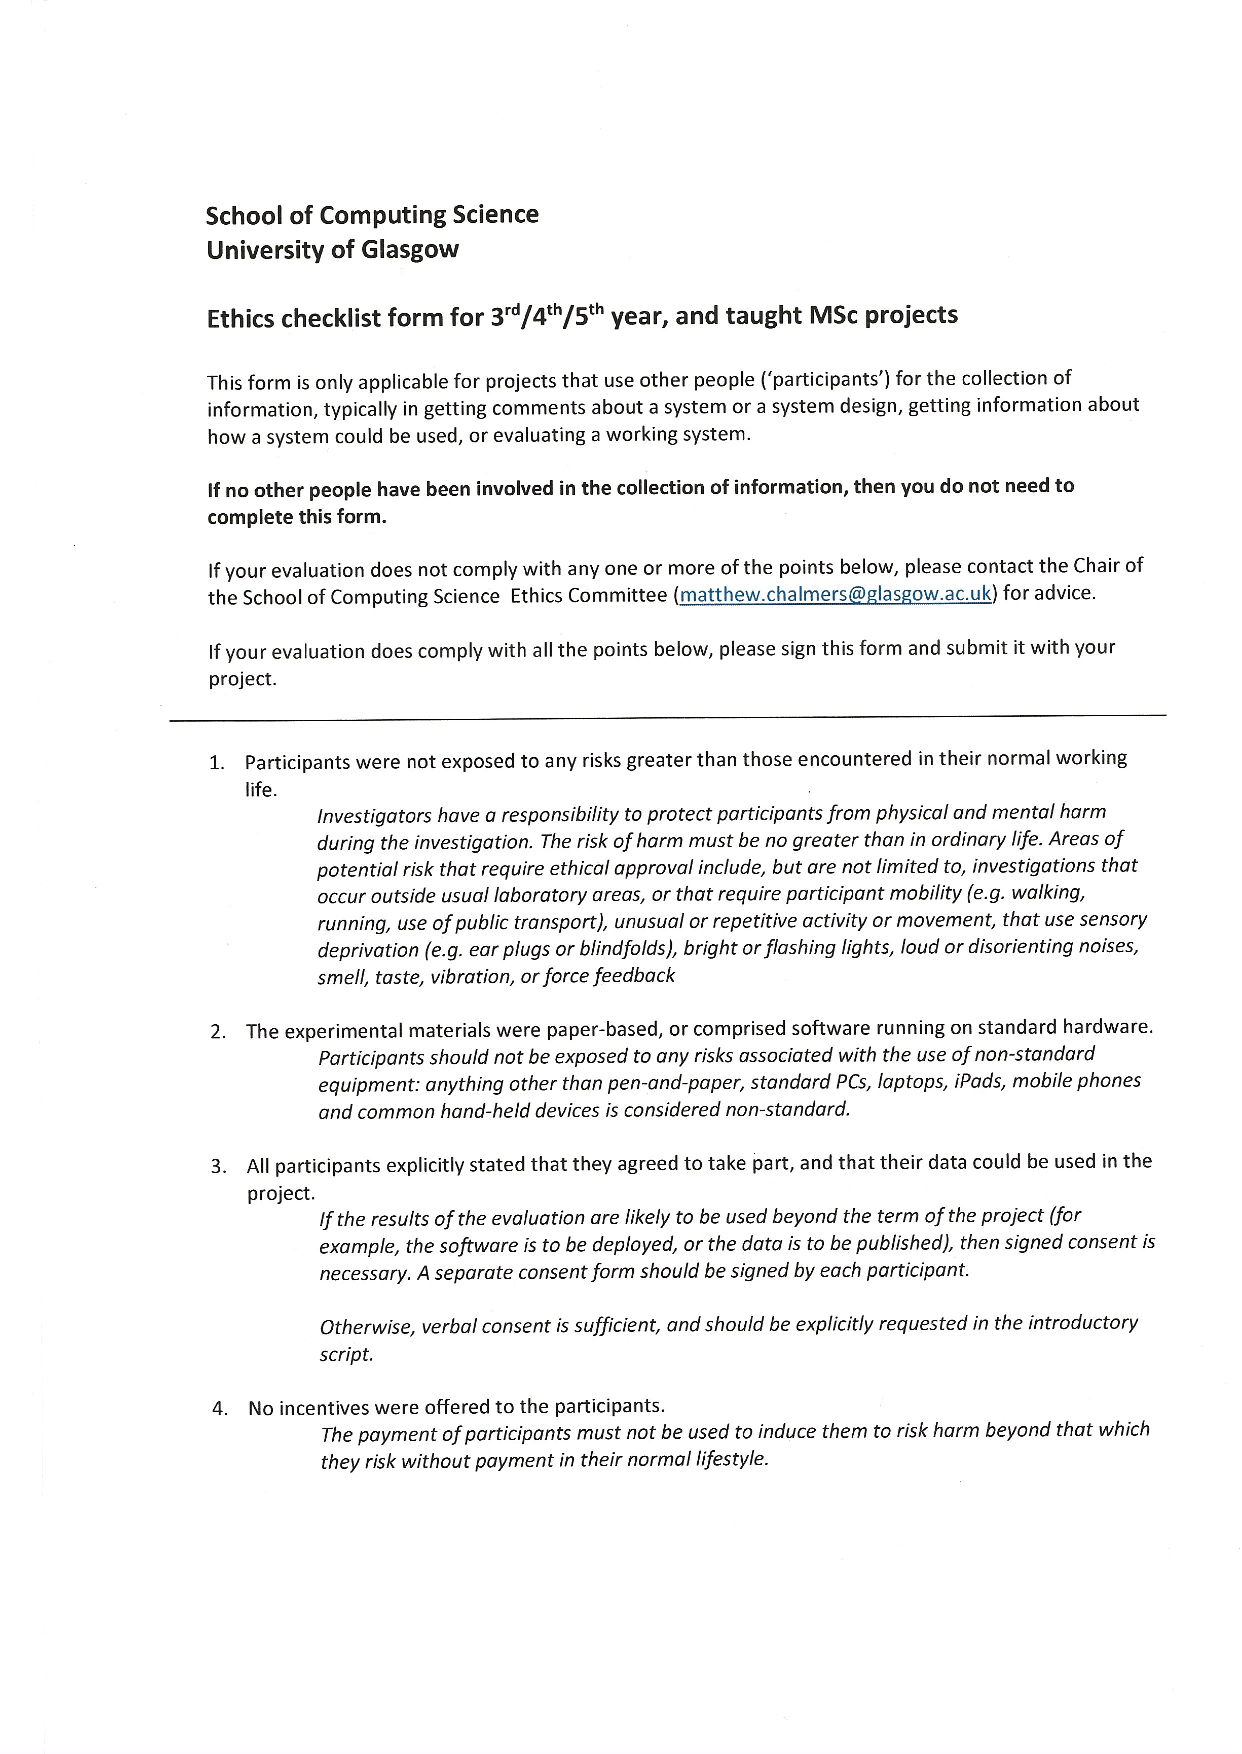
\includepdf[pages=-]{checklist.pdf}
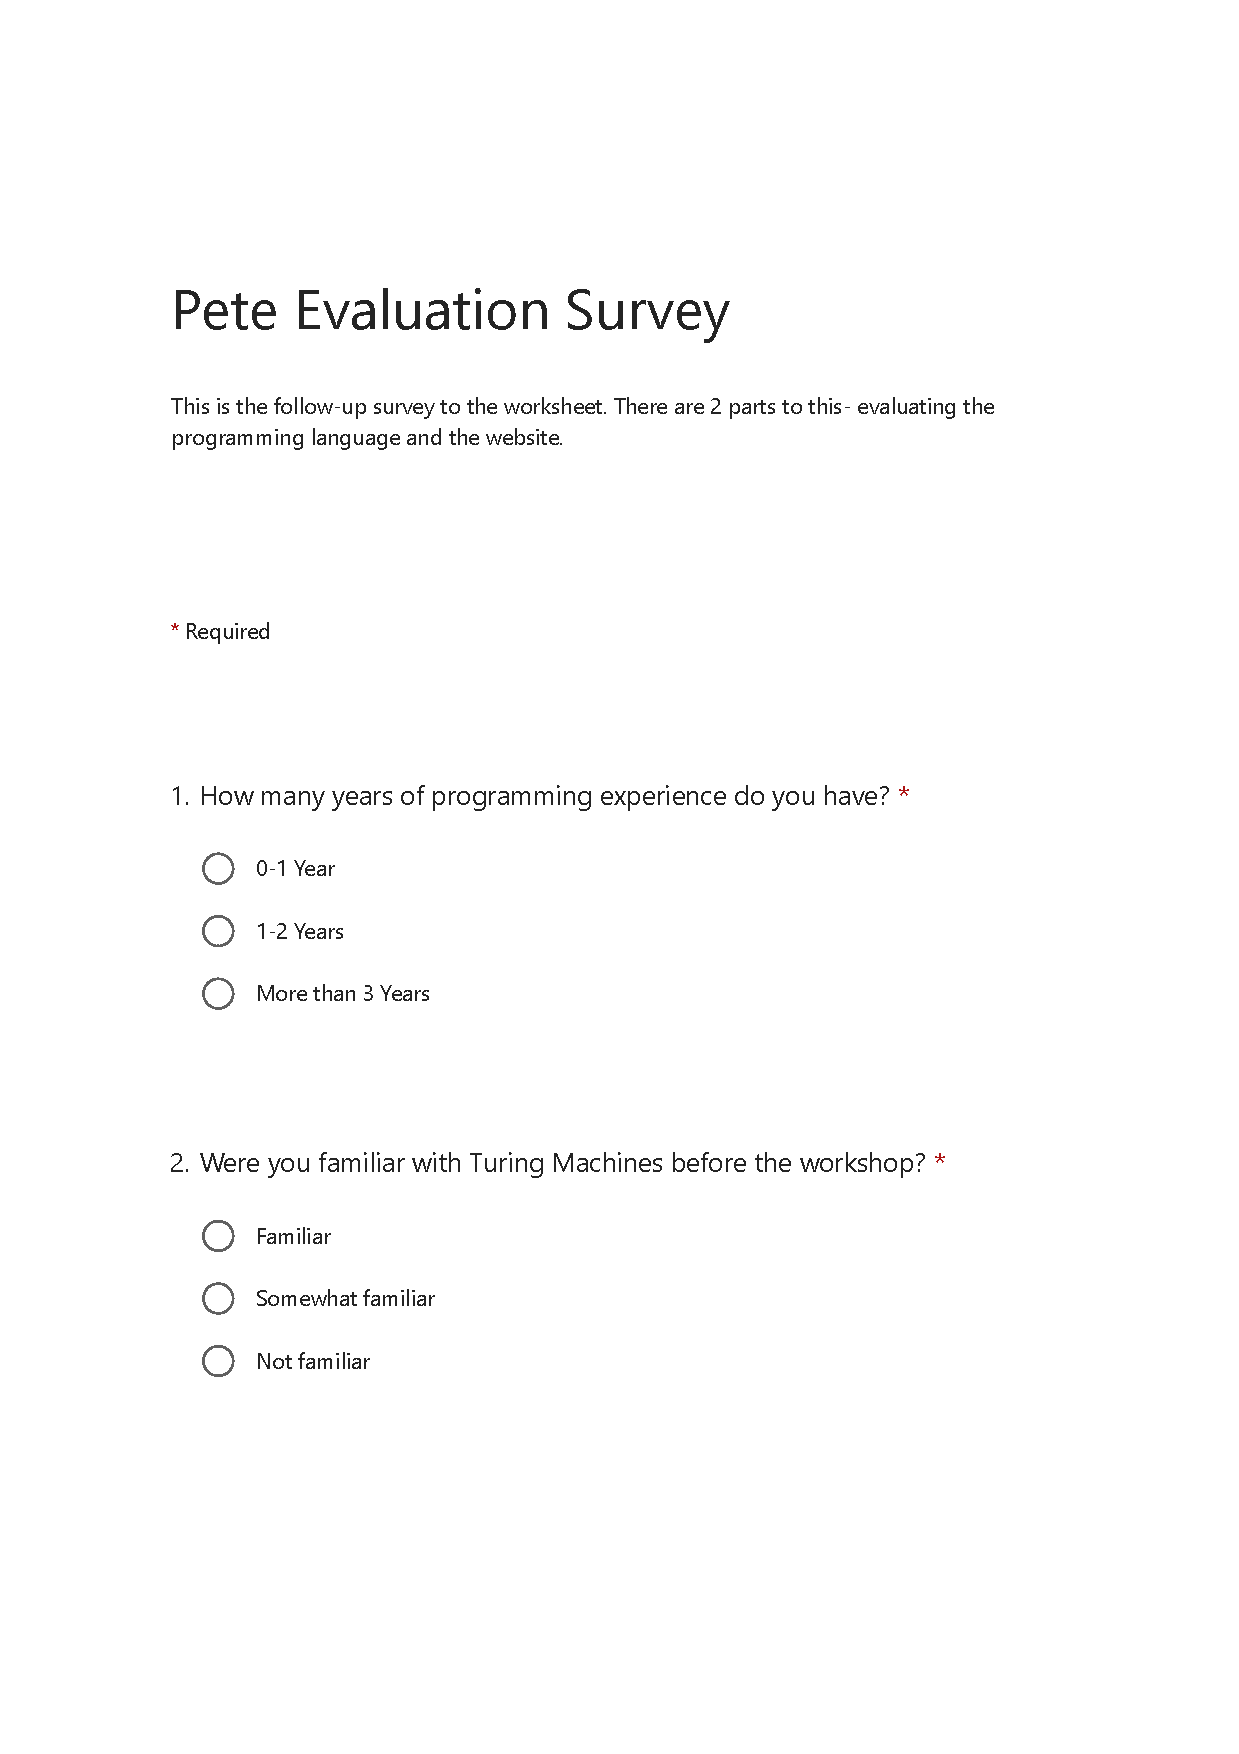
\includepdf[pages=-]{survey.pdf}

\end{appendices}
% \begin{appendices}
%     \documentclass{article}
\usepackage[utf8]{inputenc}
\usepackage{amsmath, amssymb, amsthm}
\usepackage{float}

\usepackage{listings}
\usepackage{xcolor}

\usepackage{tikz}
\usepackage{float}

\theoremstyle{definition}
\newtheorem{rules}{Rule}[section]
\newtheorem{definition}[rules]{Definition}
\newtheorem{remark}[rules]{Remark}
\newtheorem{example}[rules]{Example}

\definecolor{codegreen}{rgb}{0,0.6,0}
\definecolor{codegray}{rgb}{0.5,0.5,0.5}
\definecolor{codepurple}{rgb}{0.58,0,0.82}
\definecolor{backcolour}{rgb}{0.95,0.95,0.92}

\lstdefinestyle{thestyle}{
    backgroundcolor=\color{backcolour},
    basicstyle=\ttfamily\footnotesize,
    keywordstyle=\color{red!80}\bfseries,
    ndkeywordstyle=\color{blue!80}\bfseries,
    identifierstyle=\color{black},
    commentstyle=\color{codegreen},
    stringstyle=\color{codepurple},
    breakatwhitespace=false,
    breaklines=true,
    captionpos=b,
    keepspaces=true,
    numberstyle=\tiny\color{codegray},
    numbers=left,
    numbersep=2pt,
    showspaces=false,
    showstringspaces=false,
    showtabs=false,          
    tabsize=2
}

\lstset{style=thestyle}

\lstdefinelanguage{TML}{ 
    keywords={changeto, move, goto, if, switch, while, module, accept, reject, halt, alphabet},
    ndkeywords={left, right, tapehead, blank},
    sensitive=true,
    comment=[l]{//},
    morecomment=[s]{/*}{*/},
    morestring=[b]',
    morestring=[b]"
}

\title{TML Specification}
\author{Pete Gautam}

\begin{document}
    \maketitle
    \begin{abstract}
        This document contains the specification of the TM programming language (called Turing Machine Language, or TML), and how it can be used to change the state of a tape. In the first section, we discuss TML rules (the EBNF and contextual rules), and give examples of valid and invalid TML programs. In the second section, we define tapes and how a TML program can be executed on a tape. This section also includes some examples of executing a TM program on a given tape.
    \end{abstract}

    \section{TML rules}
    In this section, we define the rules that a valid program in TML should obey. First, the following is the specification of the TML in EBNF:
    \begin{align*}
        \textit{program} &= \textit{alphabet} \ \textit{module}^+ \\
        \textit{alphabet} &= \texttt{alphabet} \ \texttt{=} \ \texttt{\{} \ \textit{seq-val} \ \texttt{\}} \\
        \textit{module} &= \texttt{module} \ \textit{id} \ \texttt{\{} \ \textit{block}^+ \ \texttt{\}} \\
        \textit{block} &= \textit{basic-block} \ | \ \textit{switch-block} \\
        \textit{switch-block} &= \texttt{switch tapehead \{} \ \textit{case-block}^+ \ \texttt{\}} \\
        \textit{case-block} &= \textit{if-block} \ | \ \textit{while-block} \\
        \textit{if-block} &= \texttt{if} \ \textit{seq-val} \ \texttt{\{} \textit{block}^+ \texttt{\}} \\
        \textit{while-block} &= \texttt{while} \ \textit{seq-val} \ \texttt{\{} \ \textit{core-com}^+ \ \texttt{\}} \\
        \textit{basic-block} &= (\textit{core-com} \ | \ \textit{flow-com})^+ \\
        \textit{core-com} &= \texttt{move} \ \textit{direction} \ | \ \texttt{changeto} \ \textit{value} \\
        \textit{flow-com} &= \texttt{goto} \ \textit{id} \ | \ \textit{terminate} \\
        \textit{terminate} &= \texttt{reject} \ | \ \texttt{accept} \\
        \textit{direction} &= \texttt{left} \ | \ \texttt{right} \\
        \textit{seq-val} &= (\textit{value}^* \texttt{,}) \ \textit{value} \\
        \textit{value} &= \texttt{blank} \ | \ \texttt{a} \ | \ \texttt{b} \ | \ \texttt{c} \ | \ \dots \ | \ \texttt{z} \ | \ \texttt{0} \ | \ \texttt{1} \ | \ \dots \ | \ \texttt{9} \\
        \textit{id} &= (\texttt{a} \ | \ \texttt{b} \ | \ \texttt{c} \ | \ \dots \ | \ \texttt{z} \ | \ \texttt{A} \ | \ \texttt{B} \ | \ \texttt{C} \ | \ \dots \ | \ \texttt{Z})^+
    \end{align*}
    
    Next, we analyse the rules of a TML program.
    \begin{rules}
        A valid TML program is composed of the \emph{alphabet}, followed by one or more \emph{modules}.
    \end{rules}
    \begin{rules}
        A module contains a collection of a \emph{blocks} (a specific sequence of commands). There are two types of blocks- \emph{basic blocks} and \emph{switch blocks}.
    \end{rules}
    \begin{rules}
        A basic block consists of \emph{basic commands} (\textit{changeto}, \textit{move} or \textit{flow} command). A basic block consists of at least one basic command, but it is not necessary for a basic block to be composed of all the basic commands. If multiple commands are present in a basic block, they must be in the following order- \textit{changeto}, \textit{move} and \textit{flow} command.
    \end{rules}
    \begin{example}
        The following is a simple TML program:
\begin{lstlisting}[language=TML]
alphabet = {"a", "b"}
module simple {
    changeto blank
    move right
    changeto a
    move left
    accept
}
\end{lstlisting}
    It is composed of a single module, called \texttt{simple}. The module has 2 basic blocks- lines 3-4, and lines 5-7.
    \end{example}
    \begin{remark}
        In the example above, we could have also said that there were 5 basic blocks, one in each line from line 3 to line 7. If it is possible for us to break a module into blocks in different ways, we always choose the one that ends up with the fewest number of blocks. In this case, we cannot have just one block since lines 3-5 do not form a basic block- there are two \textit{changeto} commands. So, we have 2 basic blocks above.
    \end{remark}
    
    \begin{rules}
        A \emph{switch block} consists of a single switch statement. A switch statement must contain precisely one case (\textit{if} or \textit{while} command) for each of the letter in the alphabet, including the \texttt{blank} letter. The first block of a case block must be a basic block.
    \end{rules}
    \begin{rules}
        The body of an \textit{if} command can be composed of multiple blocks. These blocks can be both basic blocks and switch blocks.
    \end{rules}
    \begin{rules}
        The body of a \textit{while} command must be composed of a single basic block. The basic block cannot have a \textit{flow} command. Further, a switch block must be the final block present; it cannot be followed by any other block, basic or switch.
    \end{rules}
    
    \begin{example}
        The following is another TML program:
\begin{lstlisting}[language=TML]
alphabet = {"0", "1"}
module isEven {
    switch tapehead {
        while 0, 1 {
            move right
        } if blank {
            move left
            switch tapehead {
                if 0 {
                    accept
                } if 1, blank {
                    reject
                }
            }
        }
    }
}
\end{lstlisting}
    It is composed of a single module \texttt{isEven}. The module has:
    \begin{itemize}
        \item a switch block at lines 3-16;
        \item a basic block at line 5;
        \item a basic block at line 7;
        \item a nested switch block at lines 8-14;
        \item a basic block at line 10; and
        \item a basic block at line 12.
    \end{itemize}
    \end{example}
    \newpage

    \section{TML execution}
    In this section, we discuss how a valid TML program can execute a tape. The tape we will be using has infinite spaces in both directions.
    \begin{definition}
        Let $\Sigma$ be an alphabet. A \emph{tape $T$ on $\Sigma$} is a function $T: \mathbb{Z} \to \Sigma^+$, where $\Sigma^+ = \Sigma \cup \{\texttt{blank}\}$.
    \end{definition}
    \begin{remark}
        A valid TML program always specifies the alphabet. This corresponds to the alphabet $\Sigma$ used in the tape.
    \end{remark}
    \noindent Although there are many possible tapes, we will only be interested in tapes that obey some rules.
    \begin{definition}
        Let $\Sigma$ be an alphabet and let $T$ be a tape on $\Sigma$. Then, $T$ is a \emph{valid tape} if only finitely many symbols on $T$ are not \texttt{blank}, and all the values that can be non-\texttt{blank} are non-\texttt{blank}. That is, there exist integers $a, b$ such that for all $x \in \mathbb{Z}$, $T(x)$ is not \texttt{blank} if and only $x \geq a$ and $x \leq b$.
    \end{definition}
    \begin{remark}
        In a valid tape, there are only finitely many values that are non-\texttt{blank} and there is no gap between any two non-\texttt{blank} values.
    \end{remark}
    \begin{remark}
        We require the tape to have finitely many non-\texttt{blank} entries so that we start execution with the tapehead at the first non-\texttt{blank} entry. Moreover, this ensures that going from the start of the tape to the end does not create an infinite loop- this is a very common procedure. If we allowed for infinitely many non-\texttt{blank} entries, we would need to specify where the initial location of the tapehead is. Moreover, there would be much fewer programs that we could write which are guaranteed to terminate.
    \end{remark}
    \begin{remark}
        A valid tape can always be represented as an illustration. For instance, consider the following valid tape $T$ on $\{0, 1\}$:
        \[T(x) = \begin{cases}
            0 & x \in \{1, 3, 4\} \\
            1 & x \in \{2\} \\
            \texttt{blank} & \text{otherwise}.
        \end{cases}\]
        Then, an illustration of the tape is:
        \begin{figure}[H]
            \centering
            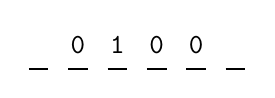
\begin{tikzpicture}
                \draw[thick] (-0.25, 0) -- (0, 0);
                \foreach \x[count=\i] in {0, 1, 0, 0} {
                    \draw[thick] (\i*0.5-0.25, 0) -- (\i*0.5, 0);
                    \node at (\i*0.5-0.125, 0.3) {\texttt{\x}};
                }
                \draw[thick] (2.25, 0) -- (2.5, 0);
            \end{tikzpicture}
            \caption{The tape as a diagram.}
        \end{figure}
        \noindent Only the non-\texttt{blank} values are represented. Blank ones are represented by empty lines.
    \end{remark}
    \begin{remark}
        More than one tape definition can result in the same diagram. In the case above, the following tape $S$ on $\{0, 1\}$ also has the same diagram.
        \[S(x) = \begin{cases}
            0 & x \in \{0, 2, 3\} \\
            1 & x \in \{1\} \\
            \texttt{blank} & \text{otherwise}.
        \end{cases}\]        
    \end{remark}
    \begin{example}
Consider the following TML program:
\begin{lstlisting}[language=TML]
alphabet = {"a", "b"}
module isSecondValueA {
    move right
    switch tapehead {
        if a {
            accept
        } if b, blank {
            reject
        }
    }
}
\end{lstlisting}
    The following is a valid tape for the program:
    \begin{figure}[H]
        \centering
        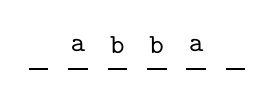
\begin{tikzpicture}
            \draw[thick] (-0.25, 0) -- (0, 0);
            \foreach \x[count=\i] in {a, b, b, a} {
                \draw[thick] (\i*0.5-0.25, 0) -- (\i*0.5, 0);
                \node at (\i*0.5-0.125, 0.3) {\texttt{\x}};
            }
            \draw[thick] (0.5*5-0.25, 0) -- (0.5*5, 0);
        \end{tikzpicture}
    \end{figure}
    \end{example}

    Now, we will define how we can execute a TML program on a valid tape.
    \begin{definition}
        Let $P$ be a TML program, let $T$ be a valid tape for the program with $i$ the smallest integer such that $T(i)$ is not \texttt{blank} ($i$ is the initial \emph{tapehead index} and $T(i)$ the initial \textit{tapehead value}). We \emph{execute $P$ on $T$} by constructing (countable) different tapes until execution is terminated. We first take the given tape and the tapehead index and execute it using the first block $b$ in the first module of $P$ to construct the next tape $T'$ and next tapehead index $i'$. This is done as follows:
        \begin{itemize}
            \item if the block is a switch block, we take the first block from the case corresponding to the tapehead value- now, we must have a basic block;
            \item if there is a \textit{changeto} \texttt{val} command in the basic block, the next tape $T'$ is given by 
            \[T'(x) = \begin{cases}
                \texttt{val} & x = i \\
                T(x) & \text{otherwise}.
            \end{cases}\]
            If the \textit{changeto} command is missing, then the tapehead $T' = T$.
            \item if there is a \textit{move} \texttt{dir} command in the basic block, the next tapehead index is given by:
            \[i' = \begin{cases}
                i+1 & \texttt{dir} = \texttt{right} \\
                i-1 & \texttt{dir} = \texttt{left}.
            \end{cases}\]
            If the \textit{move} command is missing, then $i' = i-1$.
            \item we either terminate or determine the next block $b'$ to execute (in decreasing precedence):
            \begin{itemize}
                \item if the block is the body of a while case block, then $b' = b$, i.e. we execute this switch block again (not necessarily the same case block); 
                \item if the block contains a terminating \textit{flow} command, we terminate and return the terminated state;
                \item if the block contains a \textit{goto} \texttt{mod} command, then $b'$ is the first block of the module \texttt{mod};
                \item if the block is not the final block in the module, then $b'$ is next block in this module;
                \item otherwise, we terminate and return the state \texttt{reject}.
            \end{itemize}
        \end{itemize}
        If execution is not terminated, we execute the block $b'$ with the new tape $T'$ and a new tapehead index $i'$.
    \end{definition}
    \begin{remark}
        By construction, for a valid program, precisely one of the 5 possible step applies when choosing the next block to execute or terminate.
    \end{remark}
    
    \begin{example}
        Consider the following TML program:
\begin{lstlisting}[language=TML]
alphabet = {"a", "b"}
module palindrome {
    switch tapehead {
        if blank {
            accept
        } if a {
            changeto blank
            move right
            switch tapehead {
                while a, b {
                    move right
                } if blank {
                    move left
                    switch tapehead {
                        if blank, a {
                            changeto blank
                            move left
                            goto restart
                        } if b {
                            reject
                        }
                    }
                }
            }
        }  if b {
            changeto blank
            move right
            switch tapehead {
                while a, b {
                    move right
                } if blank {
                    move left
                    switch tapehead {
                        if blank, b {
                            changeto blank
                            move left
                            goto restart
                        } if a {
                            reject
                        }
                    }
                }
            }
        }
    }
}
module restart {
    switch tapehead {
        while a, b {
            move left
        } if blank {
            move right
            goto palindrome
        }
    }
}
\end{lstlisting}
    We will execute the program on the following tape.
    \begin{figure}[H]
        \centering
        \begin{tikzpicture}
            \draw[thick] (-0.25, 0) -- (0, 0);
            \foreach \x[count=\i] in {a, b, a} {
                \draw[thick] (\i*0.5-0.25, 0) -- (\i*0.5, 0);
                \node at (\i*0.5-0.125, 0.3) {\texttt{\x}};
            }
            \draw[thick] (1.75, 0) -- (2, 0);
    
            \draw[->, thick] (0.375, -0.5) -- (0.375, -0.1);
        \end{tikzpicture}
    \end{figure}
    \noindent The arrow points to the tapehead value. We first execute the switch block at \texttt{palindrome}. Since the tapehead value is \texttt{a}, we execute the basic block at lines 7-8. So, we change the tapehead value to \texttt{blank}, and the tapehead moves to the right by one step. Since this is an \textit{if}-block, without a flow command, and there is a block following this one, the next block to be executed is the switch block at lines 9-24. Now, the current tape is the following.
    \begin{figure}[H]
        \centering
        \begin{tikzpicture}
            \draw[thick] (-0.25, 0) -- (0, 0);
            \foreach \x[count=\i] in {b, a} {
                \draw[thick] (\i*0.5-0.25, 0) -- (\i*0.5, 0);
                \node at (\i*0.5-0.125, 0.3) {\texttt{\x}};
            }
            \draw[thick] (1.25, 0) -- (1.5, 0);
    
            \draw[->, thick] (0.375, -0.5) -- (0.375, -0.1);
        \end{tikzpicture}
    \end{figure}
    \noindent The current block is a switch block. The tapehead value is \texttt{b}, so we are at the \textit{while} command at line 11. The basic block here only contains a \textit{move} command. So, we leave the tape as is, and the tapehead moves to the right once. This is a \textit{while} command, so the next block to execute is still this switch block. The current tape state is the following.
    \begin{figure}[H]
        \centering
        \begin{tikzpicture}
            \draw[thick] (-0.25, 0) -- (0, 0);
            \foreach \x[count=\i] in {b, a} {
                \draw[thick] (\i*0.5-0.25, 0) -- (\i*0.5, 0);
                \node at (\i*0.5-0.125, 0.3) {\texttt{\x}};
            }
            \draw[thick] (1.25, 0) -- (1.5, 0);
    
            \draw[->, thick] (0.875, -0.5) -- (0.875, -0.1);
        \end{tikzpicture}
    \end{figure}
    \noindent The current block is still a switch block. The tapehead value is \texttt{a}, so we execute the same \textit{while} command at line 11. Moreover, the next block to execute is still the switch block. Now, the current tape state is the following.
    \begin{figure}[H]
        \centering
        \begin{tikzpicture}
            \draw[thick] (-0.25, 0) -- (0, 0);
            \foreach \x[count=\i] in {b, a} {
                \draw[thick] (\i*0.5-0.25, 0) -- (\i*0.5, 0);
                \node at (\i*0.5-0.125, 0.3) {\texttt{\x}};
            }
            \draw[thick] (1.25, 0) -- (1.5, 0);
    
            \draw[->, thick] (1.375, -0.5) -- (1.375, -0.1);
        \end{tikzpicture}
    \end{figure}
    \noindent For the third time, we are executing the same switch block. Now, however, the tapehead value is \texttt{blank}, so we execute the first block of the \textit{if} command at line 13. Since this is an \textit{if} command and this is not the last block in the if command, the next block to execute is the switch block at lines 14-22.
    \begin{figure}[H]
        \centering
        \begin{tikzpicture}
            \draw[thick] (-0.25, 0) -- (0, 0);
            \foreach \x[count=\i] in {b, a} {
                \draw[thick] (\i*0.5-0.25, 0) -- (\i*0.5, 0);
                \node at (\i*0.5-0.125, 0.3) {\texttt{\x}};
            }
            \draw[thick] (1.25, 0) -- (1.5, 0);
    
            \draw[->, thick] (0.875, -0.5) -- (0.875, -0.1);
        \end{tikzpicture}
    \end{figure}
    \noindent Now, the current block is a switch block. The tapehead value is \texttt{a}, so we take the basic block at lines 16-18. The value of the tapehead becomes \texttt{blank}, and the tapehead moves to the left. The next block to execute is the switch block in \texttt{restart}.
    \begin{figure}[H]
        \centering
        \begin{tikzpicture}
            \draw[thick] (-0.25, 0) -- (0, 0);
            \foreach \x[count=\i] in {b} {
                \draw[thick] (\i*0.5-0.25, 0) -- (\i*0.5, 0);
                \node at (\i*0.5-0.125, 0.3) {\texttt{\x}};
            }
            \draw[thick] (0.75, 0) -- (1, 0);
    
            \draw[->, thick] (0.375, -0.5) -- (0.375, -0.1);
        \end{tikzpicture}
    \end{figure}
    \noindent Since the current tapehead value is \texttt{b}, we execute the basic block at line 50. So, we move to the left, and the tape is left as is. Moreover, since this is a while block, the next block to execute is still the switch block.
    \begin{figure}[H]
        \centering
        \begin{tikzpicture}
            \draw[thick] (-0.25, 0) -- (0, 0);
            \foreach \x[count=\i] in {b} {
                \draw[thick] (\i*0.5-0.25, 0) -- (\i*0.5, 0);
                \node at (\i*0.5-0.125, 0.3) {\texttt{\x}};
            }
            \draw[thick] (0.75, 0) -- (1, 0);
    
            \draw[->, thick] (-0.125, -0.5) -- (-0.125, -0.1);
        \end{tikzpicture}
    \end{figure}
    \noindent Since the current tapehead state is \texttt{blank}, we execute the basic block at lines 52-53. So, we move to the right, and the tape is left as is. The next block to execute is the switch block at \texttt{palindrome}.
    \begin{figure}[H]
        \centering
        \begin{tikzpicture}
            \draw[thick] (-0.25, 0) -- (0, 0);
            \foreach \x[count=\i] in {b} {
                \draw[thick] (\i*0.5-0.25, 0) -- (\i*0.5, 0);
                \node at (\i*0.5-0.125, 0.3) {\texttt{\x}};
            }
            \draw[thick] (0.75, 0) -- (1, 0);
    
            \draw[->, thick] (0.375, -0.5) -- (0.375, -0.1);
        \end{tikzpicture}
    \end{figure}
    \noindent Since the current tapehead state is \texttt{b}, we execute the basic block at lines 26-27. So, we change the tapehead value to \texttt{blank}, move to the right. This is a while block, so the next block to be executed is still the switch block.
    \begin{figure}[H]
        \centering
        \begin{tikzpicture}
            \draw[thick] (-0.25, 0) -- (0, 0);
            \draw[thick] (0.25, 0) -- (0.5, 0);
            \draw[thick] (0.75, 0) -- (1, 0);
    
            \draw[->, thick] (0.875, -0.5) -- (0.875, -0.1);
        \end{tikzpicture}
    \end{figure}
    \noindent The current tapehead state is \texttt{blank}, so we execute the basic block at line 32. We move to the left and keep the tape as is. The next block to execute is the switch block at lines 33-41.
    \begin{figure}[H]
        \centering
        \begin{tikzpicture}
            \draw[thick] (-0.25, 0) -- (0, 0);
            \draw[thick] (0.25, 0) -- (0.5, 0);
            \draw[thick] (0.75, 0) -- (1, 0);
    
            \draw[->, thick] (0.375, -0.5) -- (0.375, -0.1);
        \end{tikzpicture}
    \end{figure}
    \noindent The current tapehead value is \texttt{blank}, so we execute the basic block at lines 35-37. We keep the tape as is, and move to the left. The next block to execute is the switch block at lines 48-55.
    \begin{figure}[H]
        \centering
        \begin{tikzpicture}
            \draw[thick] (-0.25, 0) -- (0, 0);
            \draw[thick] (0.25, 0) -- (0.5, 0);
            \draw[thick] (0.75, 0) -- (1, 0);
    
            \draw[->, thick] (-0.125, -0.5) -- (-0.125, -0.1);
        \end{tikzpicture}
    \end{figure}
    \noindent The current tapehead value is \texttt{blank}, so we execute the basic block at lines 52-53. In that case, we move to the right and go to the switch block at \texttt{palindrome}.
    \begin{figure}[H]
        \centering
        \begin{tikzpicture}
            \draw[thick] (-0.25, 0) -- (0, 0);
            \draw[thick] (0.25, 0) -- (0.5, 0);
            \draw[thick] (0.75, 0) -- (1, 0);
    
            \draw[->, thick] (0.375, -0.5) -- (0.375, -0.1);
        \end{tikzpicture}
    \end{figure}
    \noindent The current tapehead value is \texttt{blank}, so we execute the basic block at line 5. We move to the left, keep the tapehead as is, and accept the tape. In that case, the final state of the tape is the following.
    \begin{figure}[H]
        \centering
        \begin{tikzpicture}
            \draw[thick] (-0.25, 0) -- (0, 0);
            \draw[thick] (0.25, 0) -- (0.5, 0);
            \draw[thick] (0.75, 0) -- (1, 0);
    
            \draw[->, thick] (-0.125, -0.5) -- (-0.125, -0.1);
        \end{tikzpicture}
    \end{figure}
\end{example}
\end{document}

%     \include{proof_of_equivalence}
%     % \chapter{Incorrect TML Programs}

Below is a selection of incorrect TML programs, along with an explanation as to why they are incorrect.
\begin{itemize}
    \item \textbf{Invalid while block (flow command)}
\begin{lstlisting}[language=TML]
alphabet = {a, b}
module main {
    while a, b {
        accept
    }
}
\end{lstlisting}
    A while block cannot have a flow command. We know that the next block to be executed is the same block, so this doesn't make sense- are we meant to terminate or re-run the current block?

    \item \textbf{Invalid while block (multiple blocks)}
\begin{lstlisting}[language=TML]
alphabet = {a, b}
module main {
    while blank {
        move left
        move right
    }
}
\end{lstlisting}
    A while block must be composed of a single basic block. We know that a while block corresponds to a self-loop, so if we have 2 blocks, we would need another state to link to the current state. This doesn't make sense, so we can only have one block. The block must also be a simple block since we have already fixed what character the while block applies to.

    \item \textbf{Invalid switch block (first block not basic)}
\begin{lstlisting}[language=TML]
alphabet = {a, b}
module main {
    if a, blank {
        if a {
            move right
        }
    }
}
\end{lstlisting}
    The first block in a switch block must be a basic block. That is, we cannot have nested if blocks without an intermediate command. This does not make sense semantically- in the case above, we should just have a single if block for \texttt{a}.

    \item \textbf{Invalid module (flow command not final)}
\begin{lstlisting}[language=TML]
alphabet = {a, b}
module main {
    goto simple
    move left
}
module simple {
    reject
}
\end{lstlisting}
    If we have a \emph{flow}-command in a block, then it must be the final command. A \emph{flow}-command moves to terminating execution or executing a module from the start, so any command below it cannot be executed. In this case, we are moving to a different block called \texttt{simple}, so we never move \texttt{left}.

    \item \textbf{Invalid module (switch block not final)}
\begin{lstlisting}[language=TML]
alphabet = {a, b}
module a {
    if a, b {
        changeto blank
        move right
        move right
        changeto b
    } if blank {
        move left
        changeto a
        reject
    }
    accept
}
\end{lstlisting}
    If a module has a \textit{switch} block, it must be the final block. In this case, that is not the case. It is possible that the program is meant to accept if we execute the \textit{if}-block at line 3, but it is not possible to continue the \textit{if}-block at line 8- this block already ends with a flow command. So, the execution would be unclear if this was allowed.

    \item \textbf{Invalid module (invalid name)}
\begin{lstlisting}[language=TML]
alphabet = {a, b}
module accept {
    move right
}
\end{lstlisting}
    A module cannot be named \texttt{accept} or \texttt{reject}. It can be named any of the other keywords, but not \texttt{accept} or \texttt{reject}.

\end{itemize}

%     \chapter{TML Examples}
\section{Executing a TML program on a Tape}
Consider the following TML program:
\begin{lstlisting}[language=TML]
alphabet = {"a", "b"}
module palindrome {
    if blank {
        accept
    } if a {
        changeto blank
        move right
        while a, b {
            move right
        } if blank {
            move left
            if blank, a {
                changeto blank
                move left
                goto restart
            } if b {
                reject
            }
        }
    }  if b {
        changeto blank
        move right
        while a, b {
            move right
        } if blank {
            move left
            if blank, b {
                changeto blank
                move left
                goto restart
            } if a {
                reject
            }
        }
    }
}
module restart {
    while a, b {
        move left
    } if blank {
        move right
        goto palindrome
    }
}
\end{lstlisting}
We will execute the program on the following tape.
\begin{figure}[H]
    \centering
    \begin{tikzpicture}
        \draw[thick] (-0.25, 0) -- (0, 0);
        \foreach \x[count=\i] in {a, b, a} {
            \draw[thick] (\i*0.5-0.25, 0) -- (\i*0.5, 0);
            \node at (\i*0.5-0.125, 0.3) {\texttt{\x}};
        }
        \draw[thick] (1.75, 0) -- (2, 0);

        \draw[->, thick] (0.375, -0.5) -- (0.375, -0.1);
    \end{tikzpicture}
\end{figure}
\noindent The arrow points at the tapehead value. We first execute the first block in the module \texttt{palindrome}. Since the tapehead value is \texttt{a}, we execute the basic block at lines 5-20. So, we change the tapehead value to \texttt{blank}, and the tapehead moves to the right by one step. Since this is an \textit{if}-block, without a flow command, and there is a block following this one, the next block to be executed is the switch block at lines 8-19. Now, the current tape is the following.
\begin{figure}[H]
    \centering
    \begin{tikzpicture}
        \draw[thick] (-0.25, 0) -- (0, 0);
        \foreach \x[count=\i] in {b, a} {
            \draw[thick] (\i*0.5-0.25, 0) -- (\i*0.5, 0);
            \node at (\i*0.5-0.125, 0.3) {\texttt{\x}};
        }
        \draw[thick] (1.25, 0) -- (1.5, 0);

        \draw[->, thick] (0.375, -0.5) -- (0.375, -0.1);
    \end{tikzpicture}
\end{figure}
\noindent The current block is a switch block. The tapehead value is \texttt{b}, so we are at the \textit{while} command at line 9. The basic block here only contains a \textit{move} command. So, we leave the tape as is, and the tapehead moves to the right once. This is a \textit{while} command, so the next block to execute is still this switch block. The current tape state is the following.
\begin{figure}[H]
    \centering
    \begin{tikzpicture}
        \draw[thick] (-0.25, 0) -- (0, 0);
        \foreach \x[count=\i] in {b, a} {
            \draw[thick] (\i*0.5-0.25, 0) -- (\i*0.5, 0);
            \node at (\i*0.5-0.125, 0.3) {\texttt{\x}};
        }
        \draw[thick] (1.25, 0) -- (1.5, 0);

        \draw[->, thick] (0.875, -0.5) -- (0.875, -0.1);
    \end{tikzpicture}
\end{figure}
\noindent The current block is still a switch block. The tapehead value is \texttt{a}, so we execute the same \textit{while} command at line 9. Moreover, the next block to execute is still the switch block. Now, the current tape state is the following.
\begin{figure}[H]
    \centering
    \begin{tikzpicture}
        \draw[thick] (-0.25, 0) -- (0, 0);
        \foreach \x[count=\i] in {b, a} {
            \draw[thick] (\i*0.5-0.25, 0) -- (\i*0.5, 0);
            \node at (\i*0.5-0.125, 0.3) {\texttt{\x}};
        }
        \draw[thick] (1.25, 0) -- (1.5, 0);

        \draw[->, thick] (1.375, -0.5) -- (1.375, -0.1);
    \end{tikzpicture}
\end{figure}
\noindent For the third time, we are executing the same switch block. Now, however, the tapehead value is \texttt{blank}, so we execute the first block of the \textit{if} command at line 5, i.e. we move to the left. Since this is an \textit{if} command and this is not the last block in the if command, the next block to execute is the switch block at lines 12-18.
\begin{figure}[H]
    \centering
    \begin{tikzpicture}
        \draw[thick] (-0.25, 0) -- (0, 0);
        \foreach \x[count=\i] in {b, a} {
            \draw[thick] (\i*0.5-0.25, 0) -- (\i*0.5, 0);
            \node at (\i*0.5-0.125, 0.3) {\texttt{\x}};
        }
        \draw[thick] (1.25, 0) -- (1.5, 0);

        \draw[->, thick] (0.875, -0.5) -- (0.875, -0.1);
    \end{tikzpicture}
\end{figure}
\noindent Now, the current block is a switch block. The tapehead value is \texttt{a}, so we take the basic block at lines 12-16. The value of the tapehead becomes \texttt{blank}, and moves to the left. The next block to execute is the switch block in \texttt{restart}.
\begin{figure}[H]
    \centering
    \begin{tikzpicture}
        \draw[thick] (-0.25, 0) -- (0, 0);
        \foreach \x[count=\i] in {b} {
            \draw[thick] (\i*0.5-0.25, 0) -- (\i*0.5, 0);
            \node at (\i*0.5-0.125, 0.3) {\texttt{\x}};
        }
        \draw[thick] (0.75, 0) -- (1, 0);

        \draw[->, thick] (0.375, -0.5) -- (0.375, -0.1);
    \end{tikzpicture}
\end{figure}
\noindent Since the current tapehead value is \texttt{b}, we execute the basic block at line 39. So, we move to the left, and the tape is left as is. Moreover, since this is a while block, the next block to execute is still the switch block.
\begin{figure}[H]
    \centering
    \begin{tikzpicture}
        \draw[thick] (-0.25, 0) -- (0, 0);
        \foreach \x[count=\i] in {b} {
            \draw[thick] (\i*0.5-0.25, 0) -- (\i*0.5, 0);
            \node at (\i*0.5-0.125, 0.3) {\texttt{\x}};
        }
        \draw[thick] (0.75, 0) -- (1, 0);

        \draw[->, thick] (-0.125, -0.5) -- (-0.125, -0.1);
    \end{tikzpicture}
\end{figure}
\noindent Since the current tapehead state is \texttt{blank}, we execute the basic block at lines 40-43. So, we move to the left, and the tape is left as is. The next block to execute is the switch block at \texttt{palindrome}.
\begin{figure}[H]
    \centering
    \begin{tikzpicture}
        \draw[thick] (-0.25, 0) -- (0, 0);
        \foreach \x[count=\i] in {b} {
            \draw[thick] (\i*0.5-0.25, 0) -- (\i*0.5, 0);
            \node at (\i*0.5-0.125, 0.3) {\texttt{\x}};
        }
        \draw[thick] (0.75, 0) -- (1, 0);

        \draw[->, thick] (0.375, -0.5) -- (0.375, -0.1);
    \end{tikzpicture}
\end{figure}
\noindent Since the current tapehead state is \texttt{b}, we execute the basic block at lines 21-22. So, we change the tapehead value to \texttt{blank}, move to the right. This is a while block, so the next block to be executed is still the switch block.
\begin{figure}[H]
    \centering
    \begin{tikzpicture}
        \draw[thick] (-0.25, 0) -- (0, 0);
        \draw[thick] (0.25, 0) -- (0.5, 0);
        \draw[thick] (0.75, 0) -- (1, 0);

        \draw[->, thick] (0.875, -0.5) -- (0.875, -0.1);
    \end{tikzpicture}
\end{figure}
\noindent At this point, the tapehead index moves between the blank values as we move to the basic block at line 3. Then, the execution terminates and we accept the tape.

\section{Completing a TML program}
The steps to convert a TML program to complete it is the following:
\begin{enumerate}
    \item We first break each module into smaller modules so that every module has just one basic/switch block- we add a \textit{goto} command to the next module if it appeared just below this block.
    \item Then, we can convert each basic block to a switch block by just adding a single case that applies to each letter in the alphabet.
    \item Finally, we add the default values to each basic block to get a complete TML program.
\end{enumerate}

We illustrate this with an example. Assume we first have the following program.
\begin{lstlisting}[language=TML]
alphabet = {"a", "b"}
module simpleProgram {
    changeto b
    move left
    move right
    accept
}
\end{lstlisting}
After applying step 1 of completion, we get the following program.
\begin{lstlisting}[language=TML]
alphabet = {"a", "b"}
module simple1 {
    changeto b
    move left
    goto simple2
}
module simple2 {
    move right
    accept
}
\end{lstlisting}
After applying step 2, we have the following program.
\begin{lstlisting}[language=TML]
alphabet = {"a", "b"}
module simple1 {
    if a, b, blank {
        changeto b
        move left
        goto simple2
    }
}
module simple2 {
    if a, b, blank {
        move right
        accept
    }
}
\end{lstlisting}
Finally, after applying step 3, we get the following program:
\begin{lstlisting}[language=TML]
alphabet = {"a", "b"}
module simple1 {
    if a {
        changeto b
        move left
        goto simple2
    } if b {
        changeto b
        move left
        goto simple2
    } if blank {
        changeto b
        move left
        goto simple2
    }
}
module simple2 {
    if a {
        changeto a
        move right
        accept
    } if b {
        changeto b
        move right
        accept
    } if blank {
        move right
        accept
    }
}
\end{lstlisting}
This program obeys the definition of a complete program.

\section{Converting a TM to a complete TML program}
Consider the following complete TM program:
\begin{lstlisting}[language=TML]
alphabet = {"a", "b"}
module moveToEnd {
    while a {
        changeto a
        move right
    } while b {
        changeto b
        move right
    } if blank {
        changeto blank
        move left
        goto checkAFirst
    }
}
module checkAFirst {
    if a {
        changeto blank
        move left
        goto checkASecond
    } if b, blank {
        changeto blank
        move left
        reject
    }
}
module checkASecond {
    if a {
        changeto blank
        move left
        accept
    } if b, blank {
        changeto blank
        move left
        reject
    }
}
\end{lstlisting}
Then, its corresponding TM is the following:
\begin{figure}[H]
    \centering
    \begin{tikzpicture}
        \node[circle, draw=black, fill=white, inner sep=0pt, minimum size=15pt] (s0) at (-0.5, 0) {$s_0$};
        \node[circle, draw=black, fill=white, inner sep=0pt, minimum size=15pt] (s1) at (2, 0) {$s_1$};
        \node[circle, draw=black, fill=white, inner sep=0pt, minimum size=15pt] (s2) at (4, 1) {$s_2$};
        \node[circle, draw=black, fill=white, inner sep=0pt, minimum size=15pt] (sY) at (6, 1) {$s_Y$};
        \node[circle, draw=black, fill=white, inner sep=0pt, minimum size=15pt] (sN) at (6, -1) {$s_N$};
        
        \draw[-stealth] (-1.5, 0) -- (s0);
        \draw[-stealth] (s0) edge[loop above] node[align=center, text width=2cm] {$a \to a, R$ $b \to b, R$} (s0);
        \draw[-stealth] (s0) -- node[above] {$\# \to \#, L$} (s1);

        \draw[-stealth] (s1) -- node[above, rotate=25] {$a \to a, L$} (s2);
        \draw[-stealth] (s1) -- node[below, rotate=-15, pos=0.4] {$\# \to \#, L$} (sN);
        \draw[-stealth] (s1) -- node[above, rotate=-15, pos=0.4] {$b \to \#, L$} (sN);

        \draw[-stealth] (s2) -- node[above] {$\# \to \#, L$} (sY);

        \draw[-stealth] (s2) -- node[above, rotate=-45] {$b \to \#, L$} (sN);
        \draw[-stealth] (s2) -- node[below, rotate=-45] {$\# \to \#, L$} (sN);
    \end{tikzpicture}
    \caption{The TM corresponding to the program above. The state $s_0$ corresponds to the module \texttt{moveToEnd}; the state $s_1$ corresponds to the module \texttt{checkAFirst}; and the state $s_2$ corresponds to the module \texttt{checkASecond}.}
\end{figure}
%     \chapter{Evaluation Worksheet}
\section{Introduction to Turing Machine Language}
In this section, you are given some programs in Turing Machine Language (TML). They will be used to explain the syntax of the programming language and how they can be run on tapes.
\begin{itemize}
    \item \texttt{isDiv2}:
    \lstinputlisting[language=TML]{code/isDiv2.txt}
    
    \item \texttt{isDiv2Rec}:
    \lstinputlisting[language=TML]{code/isDiv2Rec.txt}

    \noindent Both \texttt{isDiv2} and \texttt{isDiv2Rec} correspond to the following Turing Machine (TM):
    \begin{figure}[H]
        \centering
        \begin{tikzpicture}
            \node[state, accepting] (q0) at (0, 0) {$q_0$};
            \node[state] (q1) at (3, 0) {$q_1$};
            \node[state, fill=green, opacity=0.6] (A) at (6, -1) {$A$};
            \node[state, fill=red, opacity=0.6] (R) at (6, 1) {$R$};

            \draw[->] (q0) edge[loop above] node {$0|1, R$} (q0);
            \draw[->] (q0) -- node[above] {$\#, L$} (q1);
            \draw[->] (q1) -- node[below left] {$0, L$} (A);
            \draw[->] (q1) -- node[above left] {$1|\#, L$} (R);
        \end{tikzpicture}
    \end{figure}
    
    \item \texttt{aNbN}:
    \lstinputlisting[language=TML]{code/aNbN.txt}

    \noindent The program \texttt{aNbN} corresponds to the following TM:
    \begin{figure}[H]
        \centering
        \begin{tikzpicture}
            \node[state, accepting] (q0) at (0, 0) {$q_0$};
            \node[state] (q1) at (0, -2) {$q_1$};
            \node[state] (q2) at (6, -2) {$q_2$};
            \node[state] (q3) at (6, 0) {$q_3$};
            \node[state, fill=green, opacity=0.6] (A) at (-3, 0) {$A$};
            \node[state, fill=red, opacity=0.6] (R) at (3, -1) {$R$};

            \draw[->] (q0) -- node[left] {$a \to \#, R$} (q1);
            \draw[->] (q0) -- node[above] {$\#, L$} (A);
            \draw[->] (q0) -- node[below] {$b, L$} (R);
            \draw[->] (q1) edge[loop below] node {$a|b, R$} (q1);
            \draw[->] (q1) -- node[below] {$\#, L$} (q2);
            \draw[->] (q2) -- node[right] {$b \to \#, L$} (q3);
            \draw[->] (q3) edge[loop above] node {$a|b, L$} (q3);
            \draw[->] (q2) -- node[above] {$a|\#, L$} (R);
            \draw[->] (q3) -- node[above] {$\#, L$} (q0);
        \end{tikzpicture}
    \end{figure}
\end{itemize}

\section{Identifying TML Programs}
In this section, you are presented with TML programs. You will be given some tape values to run the program in and decode what values the program accepts. You are encouraged to use the website to try and solve this.

\begin{enumerate}
    \item Consider the following TML Program:
    \lstinputlisting[language=TML]{code/mystery1.txt}

    \begin{enumerate}
        \item Does the program accept the values:
        \begin{enumerate}
            \item $10$ (NOTE: This is $2$ in decimal)
            \item $1$
            \item $100$ (NOTE: This is $4$ in decimal)
            \item $101$ (NOTE: This is $5$ in decimal)
            \item $110$ (NOTE: This is $6$ in decimal)
        \end{enumerate}
        \item Describe the values this program accepts.
    \end{enumerate}
    \newpage

    \item Consider the following TML program:
    \lstinputlisting[language=TML]{code/mystery2.txt}
    \begin{enumerate}
        \item Does the program accept the values:
        \begin{enumerate}
            \item $ab$
            \item $aabb$
            \item $abba$
            \item $bab$
        \end{enumerate}
        
        \item Describe the values this program accepts.
    \end{enumerate}
\end{enumerate}

\newpage

\section{Identifying TMs}
In this section, you are presented with TMs. You will be given some tape values to run the program in and decode what values the program accepts. Since the website can only execute TML programs, you are also given the TML program for the code, but it is not comprehensible like the previous programs; you will likely find it easier to understand the TM than the program (which you should do!). 
\begin{enumerate}
    \item Consider the following TM FSM:
    \begin{figure}[H]
        \centering
        \begin{tikzpicture}
            \node[state, accepting] (q0) at (0, 0) {$q_0$};
            \node[state] (q1) at (3, 0) {$q_1$};
            \node[state] (q2) at (6, 0) {$q_2$};
            \node[state, fill=green, opacity=0.6] (A) at (0, -2) {$A$};
            \node[state, fill=red, opacity=0.6] (R) at (4.5, -2) {$R$};

            \draw[->] (q0) edge[loop above] node {$0, R$} (q0);
            \draw[->] (q0) edge[bend right] node[above] {$1, R$} (q1);
            \draw[->] (q1) edge[bend right] node[above] {$1, R$} (q0);
            \draw[->] (q1) edge[bend right] node[above] {$0, R$} (q2);
            \draw[->] (q2) edge[bend right] node[above] {$0, R$} (q1);
            \draw[->] (q2) edge[loop above] node {$1, R$} (q2);
            \draw[->] (q0) edge node[left] {$\#, R$} (A);
            \draw[->] (q1) edge node[left] {$\#, R$} (R);
            \draw[->] (q2) edge node[right] {$\#, R$} (R);
        \end{tikzpicture}
    \end{figure}
    You are given a basic representation of this FSM as code in Teams. The file is called mystery3.
    \begin{enumerate}
        \item Does the TM accept the values:
        \begin{enumerate}
            \item $11$ (NOTE: This is $3$ in decimal)
            \item $10$ (NOTE: This is $2$ in decimal)
            \item $1$
            \item $110$ (NOTE: This is $6$ in decimal)
            \item $1001$ (NOTE: This is $9$ in decimal)
        \end{enumerate}
        
        \item Describe the values this program accepts.
    \end{enumerate} 
    
    \item Consider the following TM FSM:
    \begin{figure}[H]
        \centering
        \begin{tikzpicture}
            \node[state, accepting] (q0) at (3, 0) {$q_0$};
            \node[state] (q1) at (2, -2) {$q_1$};
            \node[state] (q2) at (5, -3) {$q_2$};
            \node[state] (q3) at (8, -2) {$q_3$};
            \node[state] (q7) at (6, 0) {$q_4$};
            \node[state, fill=green, opacity=0.6] (A) at (0, 0) {$A$};
            \node[state, fill=red, opacity=0.6] (R) at (5, -1) {$R$};

            \draw[->] (q0) -- node[left] {$a \to \#, R$} (q1);
            \draw[->] (q0) -- node[above] {$\#, R$} (A);
            \draw[->] (q1) edge[loop below] node {$a|b, R$} (q1);
            \draw[->] (q1) -- node[below left] {$\#, L$} (q2);
            \draw[->] (q2) -- node[below right] {$b \to \#, L$} (q3);
            \draw[->] (q3) -- node[right] {$b \to \#, L$} (q7);
            \draw[->] (q7) edge[loop right] node {$a|b, L$} (q7);
            \draw[->] (q7) -- node[above] {$\#, R$} (q0);
            \draw[->] (q2) -- node[left] {$a|\#, R$} (R);
            \draw[->] (q3) -- node[above] {$a|\#, R$} (R);
            \draw[->] (q0) -- node[below] {$b, R$} (R);
        \end{tikzpicture}
    \end{figure}
    You are given a basic representation of this FSM as code in Teams. The file is called mystery4.
    \begin{enumerate}
        \item Does this TM accept the values:
        \begin{enumerate}
            \item $ab$
            \item $abb$
            \item $aabbbb$            
            \item $bab$
            \item $abba$
        \end{enumerate}

        \item Describe the values this program accepts.
    \end{enumerate}
\end{enumerate}
\newpage


\section{Writing TML Programs}

Following a similar syntax to the code given above, write the following programs. You are free to use the website to check the accuracy of the program while writing the programs.
\begin{enumerate}
    \item divisibility by 4 in binary iteratively [HINT: Go to the end and check for 2 zeros. Allow 0 as well.]
    \item divisibility by 4 in binary, recursively.
    
    \noindent The remaining questions are optional. If you attempt them, you can answer them in the survey.
    \item strings of the form $a^n b^m c^{n+m}$
    \item strings of the form $a^n b^n c^n$
    \item HARD: check there are same number of $a$'s and $b$'s
\end{enumerate}

\section{Appendix- Links}
Below are the links to the website and the survey:
\begin{itemize}
    \item Website: \href{https://pete-g00.github.io/Turing-Machine-Language/}{Link to Website}
    \item Survey: \href{https://forms.office.com/e/Ts6nKgxWkU}{Link to Survey}
\end{itemize}

% \end{appendices}

\bibliographystyle{agsm}
\renewcommand{\thechapter}{0} 
\bibliography{l4proj}

\end{document}
